
%%%%%%%%%%%% 2 %%%%%%%%%%%%%%%%%%%%%%%%%%%%%%%%%%%%%%%%%%%%%%%%%%%%%%%%%%%%%%%%%%%%%%%%%%%
\chapter{ANITA Telescope Platform}
%%%%%%%%%%%%%%%%%%%%%%%%%%%%%%%%%%%%%%%%%%%%%%%%%%%%%%%%%%%%%%%%%%%%%%%%%%%%%%%%%%%%%%%%%%
\section{Overview}
	The ANITA telescope platform is a passive broad-band radio frequency electromagnetic field transient detector and time domain voltage digitizer.  There have been four ANITA flights at the time of this thesis, numbered one through four.  ANITA1 flew in the 2006-2007 Antarctic balloon campaign\cite{ANITA1}, ANITA2 in 2007-2008\cite{ANITA2}, ANITA3 in 2014-2015 (the topic of this thesis) and most recently ANITA4 in 2016-2017.  
	
	The main instrument structure consists of a collection of radially positioned, outwardly facing, broad-band, highly-directional quad-ridge horn antennas.  The antennas are separated into three different vertically spaced rings, with each ring separated into 16 different azimuthally facing "phi-sectors." (see Figures \ref{fig:phiSectors} and \ref{fig:ANITA3_hangtest})    These co-pointing antennas allow multiple observations of a signal event with a physical distance baseline offset between them. These antennas couple the incident electromagnetic radiation into a coaxial signal line, which is then amplified by a series of low noise-figure amplifiers, band-pass filtered via analoge compound filters into the relevant frequency bandwidth, before finally being digitized by custom on board high-speed digitizer chips and readout electronics (Figure \ref{fig:RFChainBlockDiagram}).  The digitization is self-triggered by a parallel square-law integrating power detector circuit which arrives at a decision with minimal analog waveform buffering.  After digitization, waveforms are read out via a CPCI interconnect backplane to a ruggedized conductively cooled CPU writing to on-board redundant storage devices.  The payload is capable of reading out ~50Hz of full payload waveforms with low (\textless 5\% ) deadtime to disk.  Additional position and orientation data, as well as multiple diagnostic and in-situ relevant physics measurements, are recorded and precisely time-stamped by a GPS disciplined clock.  Selections of the waveforms and housekeeping measurements are telemetered down to ground servers for in-flight diagnostics, however full recovery of the data vaults is desired for a complete analysis.  The following chapter will expand upon these systems and the theoretical basis for their design and construction.
	
	
\begin{figure}
\centering
	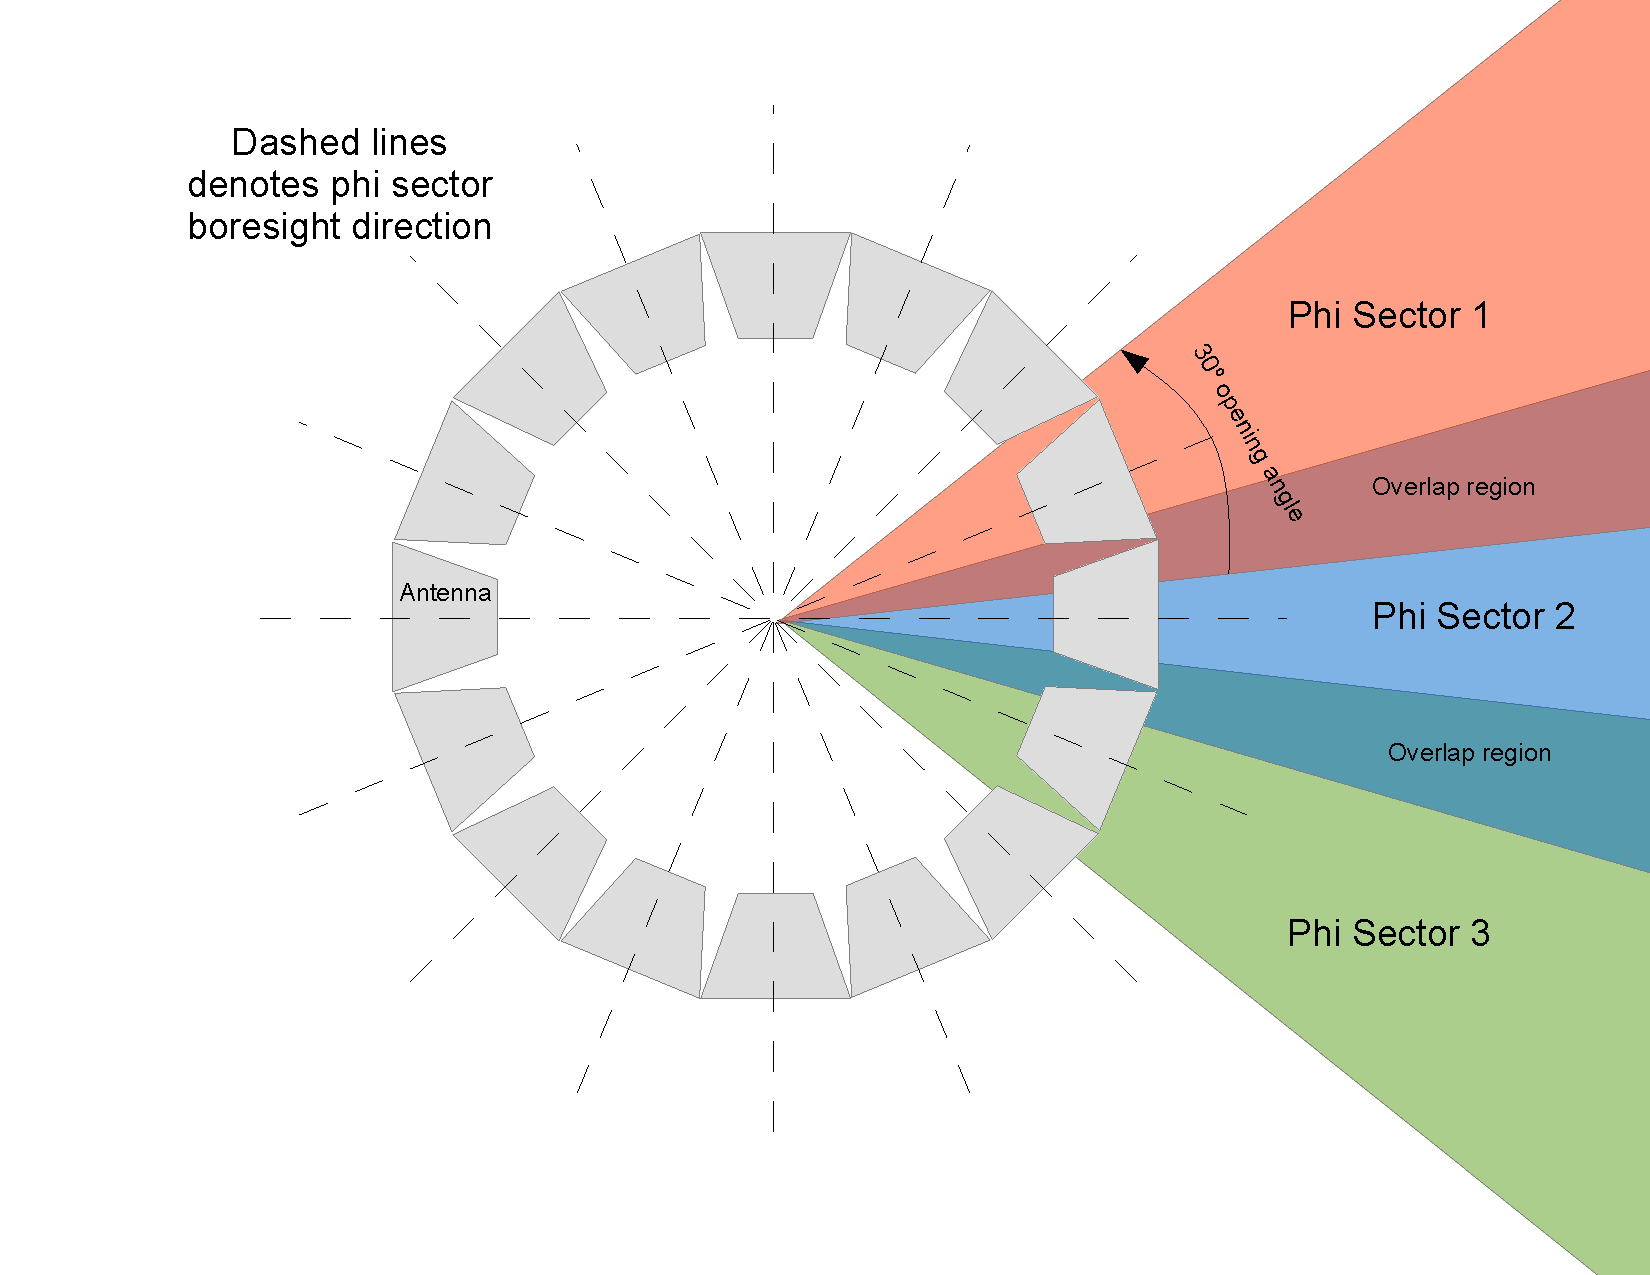
\includegraphics[width=\textwidth]{figures/phiSectors} 
	\caption{A top down diagram depicting a single ring layout of the horn antennas used to achieve complete azimuthal coverage assuming a 30$^{\circ}$  opening angle.  The antenna gain pattern is discussed further in the Calibration section.}
	\label{fig:phiSectors}
\end{figure}

	
\begin{figure}
\centering
	\includegraphics[height=0.9\textheight]{figures/ANITA3_hangtest2_annotated}
	\caption{An image of the ANITA3 telescope during the test deployment in Palestine TX, 2014.  Marked from top to bottom are two of the nine GPS antennas, the three vertically separated rings, the deployed solar panel array, and a deployed ALFA antenna.  The solar panels visible at the top of the payload are those used by the NASA Small Instrument Package (SIP).  Not visible are the ANITA instrument crate and other objects on the deck of the experiment (between middle and top antenna rings).}
	\label{fig:ANITA3_hangtest}
\end{figure}

\begin{figure}
\centering
	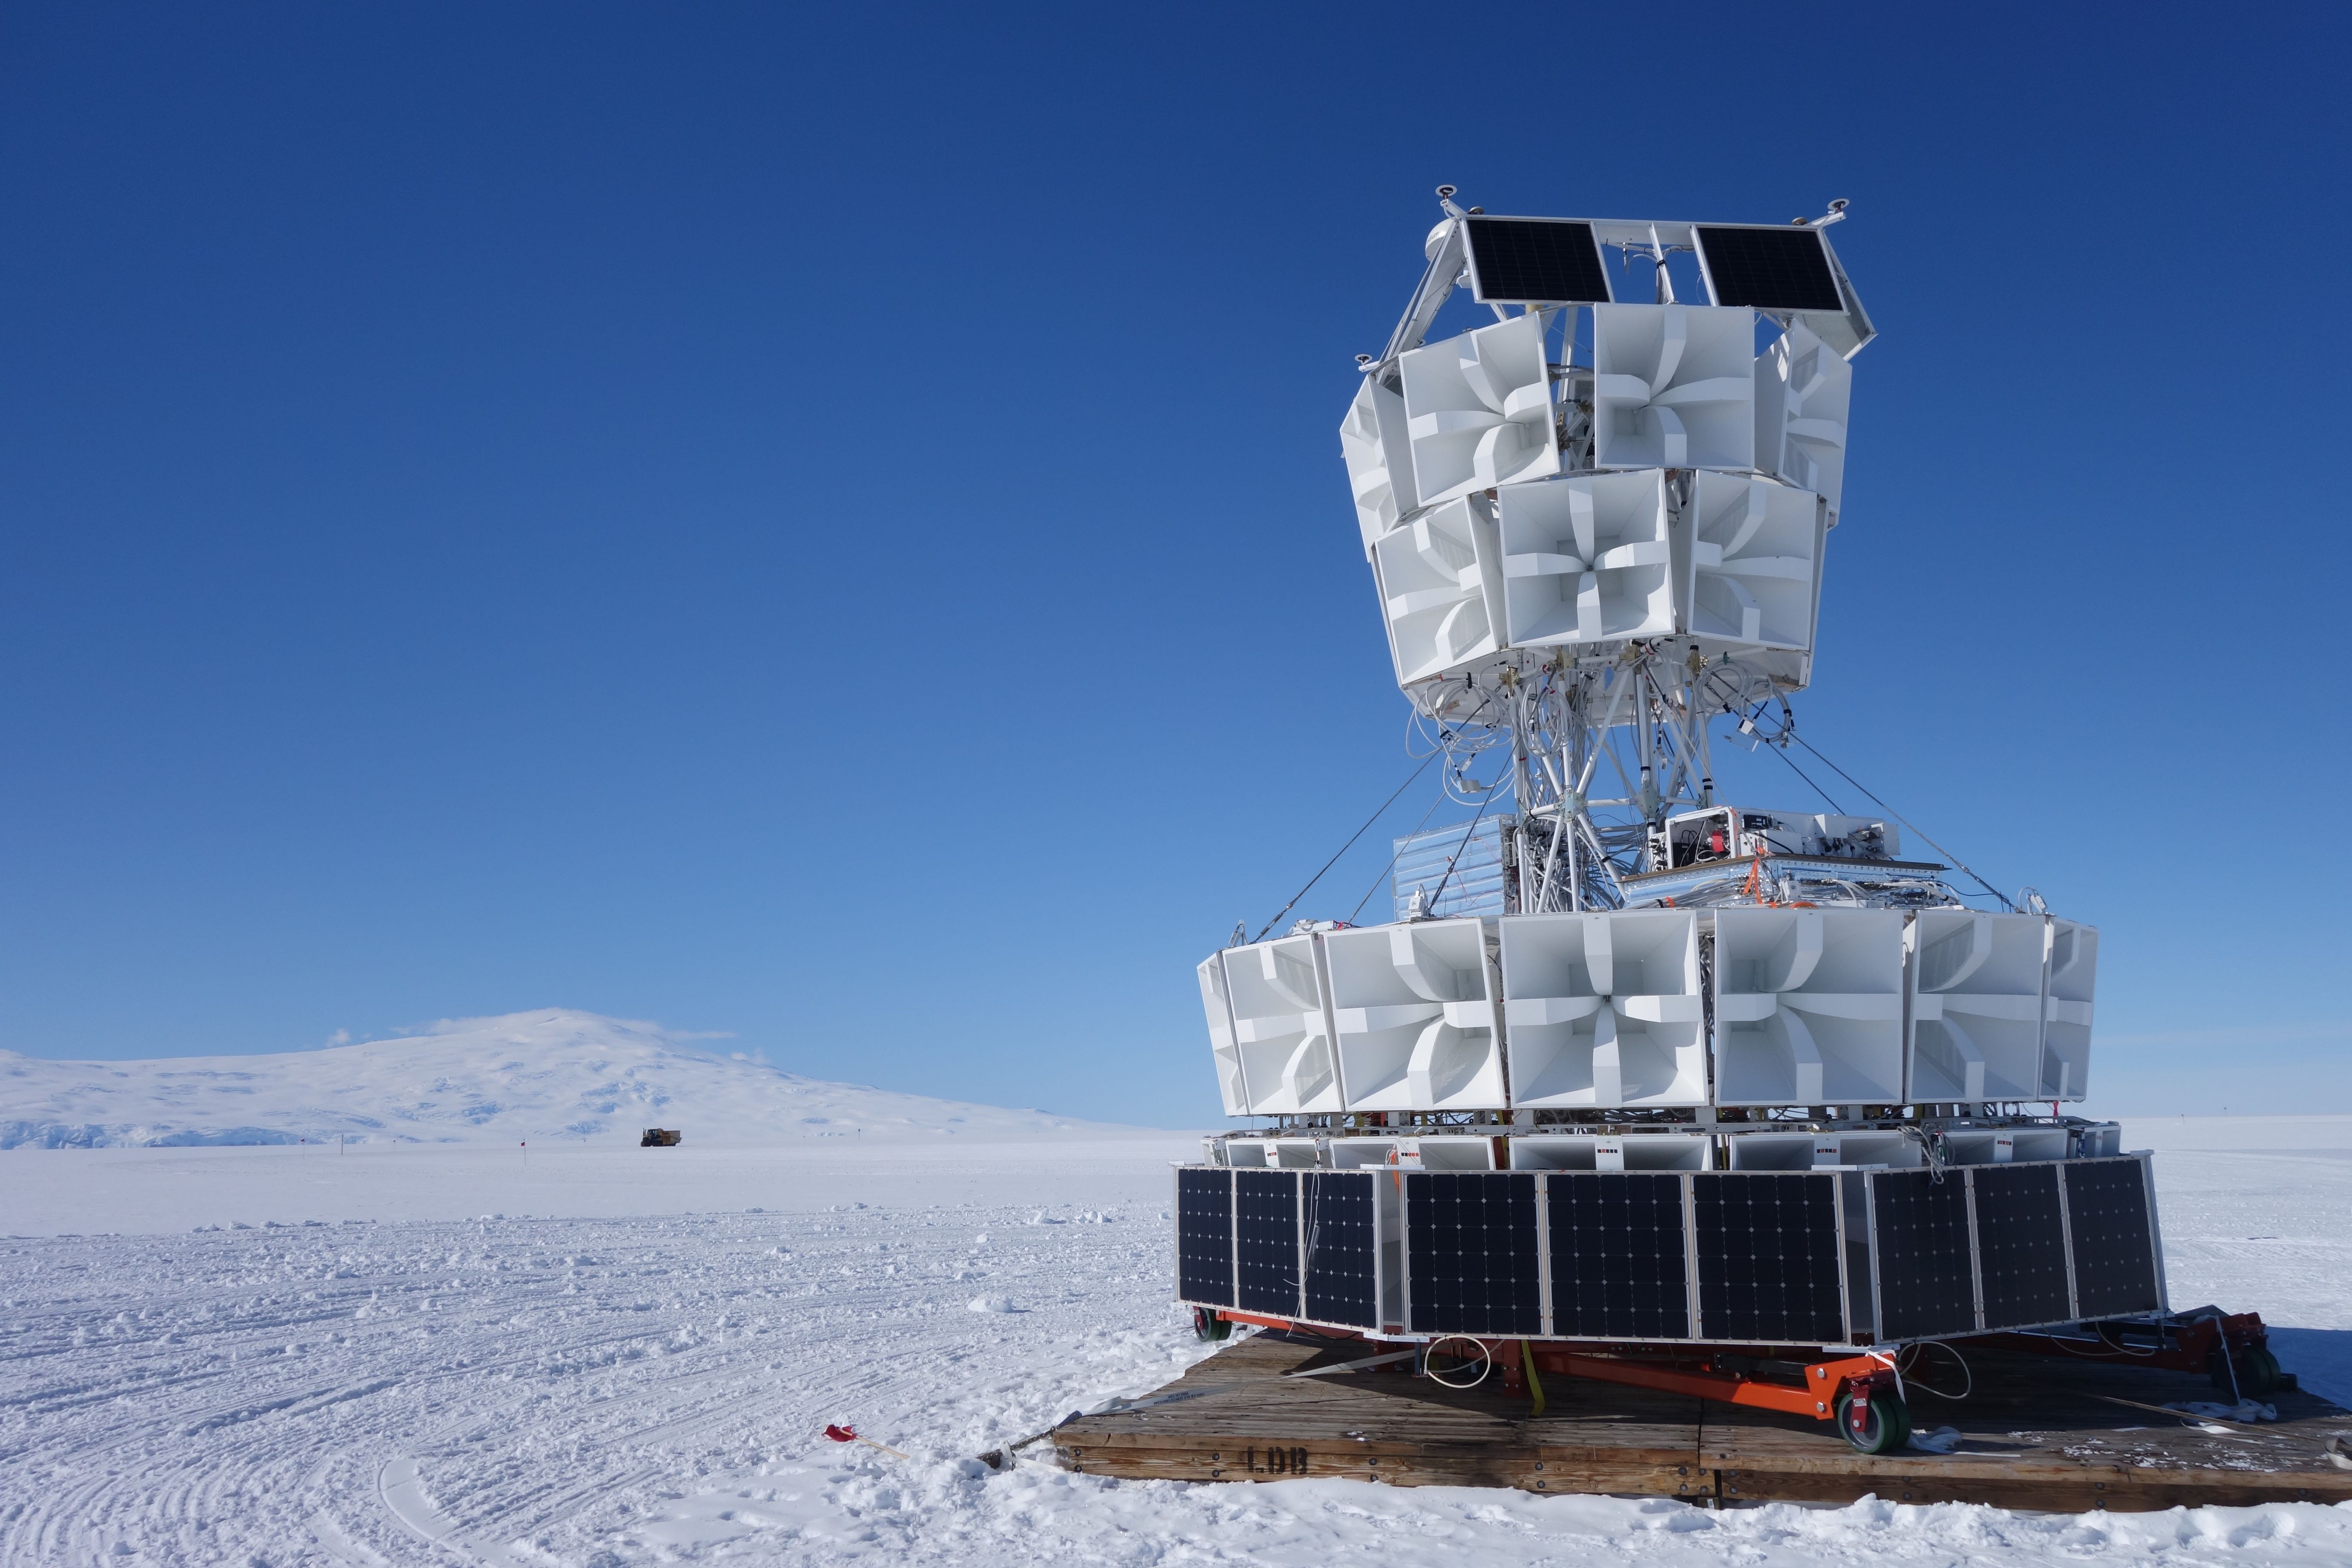
\includegraphics[width=\textwidth]{figures/ANITA3_dancefloor}
	\caption{An image of the ANITA3 during GPS calibration on the "dance-floor" at the Long Duration Balloon (LDB) facility at McMurdo Station in Antarctica prior to launch in 2014.  In the background is Mt. Erebus.  In this image the solar panels are in their retracted state, the instrument crate is visible on the left hand side of the central column, and the NASA Small Instrument Package (SIP) is visible on the right hand side. The orange structure seen under the payload is a stand used during construction and testing of the instrument.}
	\label{fig:ANITA3_dancefloor}
\end{figure}

\begin{figure}
\centering
	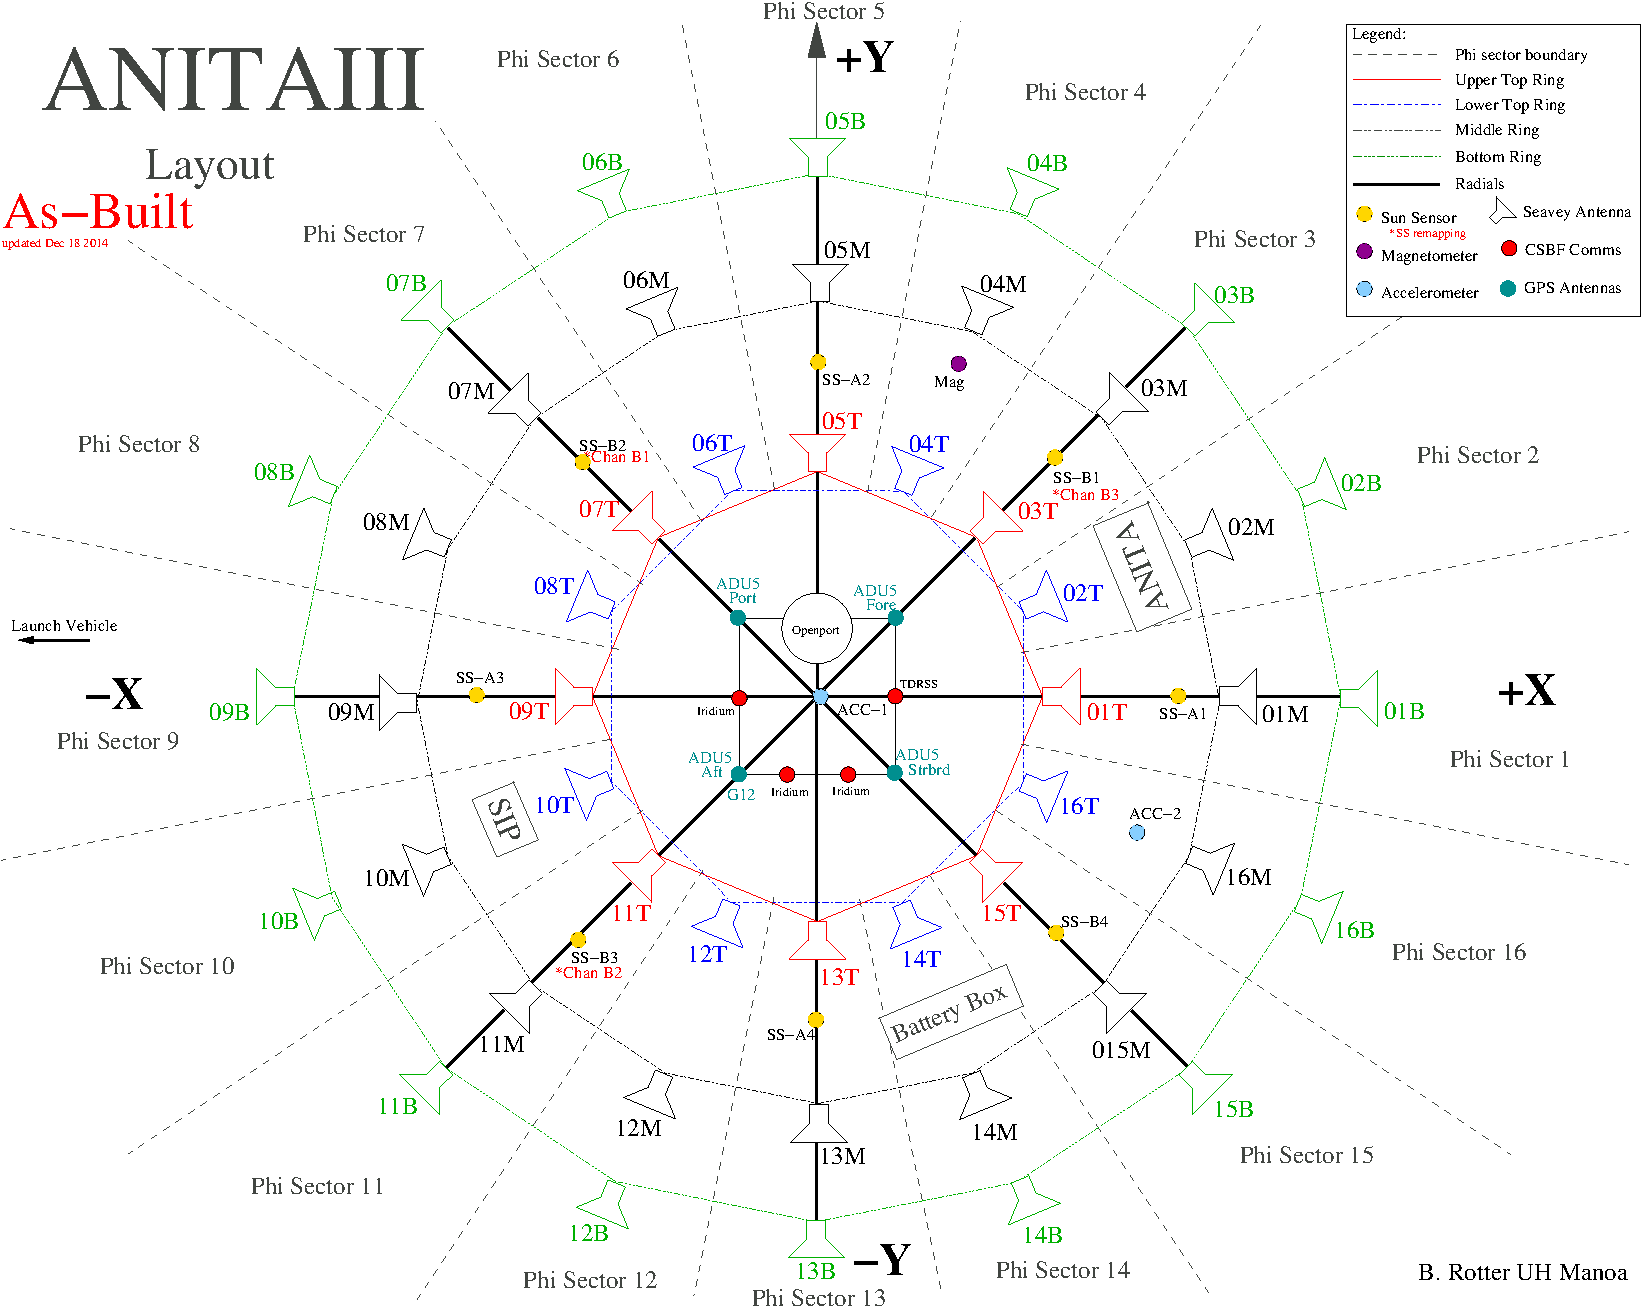
\includegraphics[width=\textwidth]{figures/ANITA3_layout_asBuilt}
	\caption{A top-down diagram detailing the locations of various components on the ANITA3 instrument as it was flown.  Visible are the locations of the NASA Small Instrument Package (SIP) and ANITA instrument box as they relate to the GPS antennas and measurement antenna phi sectors.}
	\label{fig:ANITA3_asBuilt}
\end{figure}

\begin{figure}
\centering
	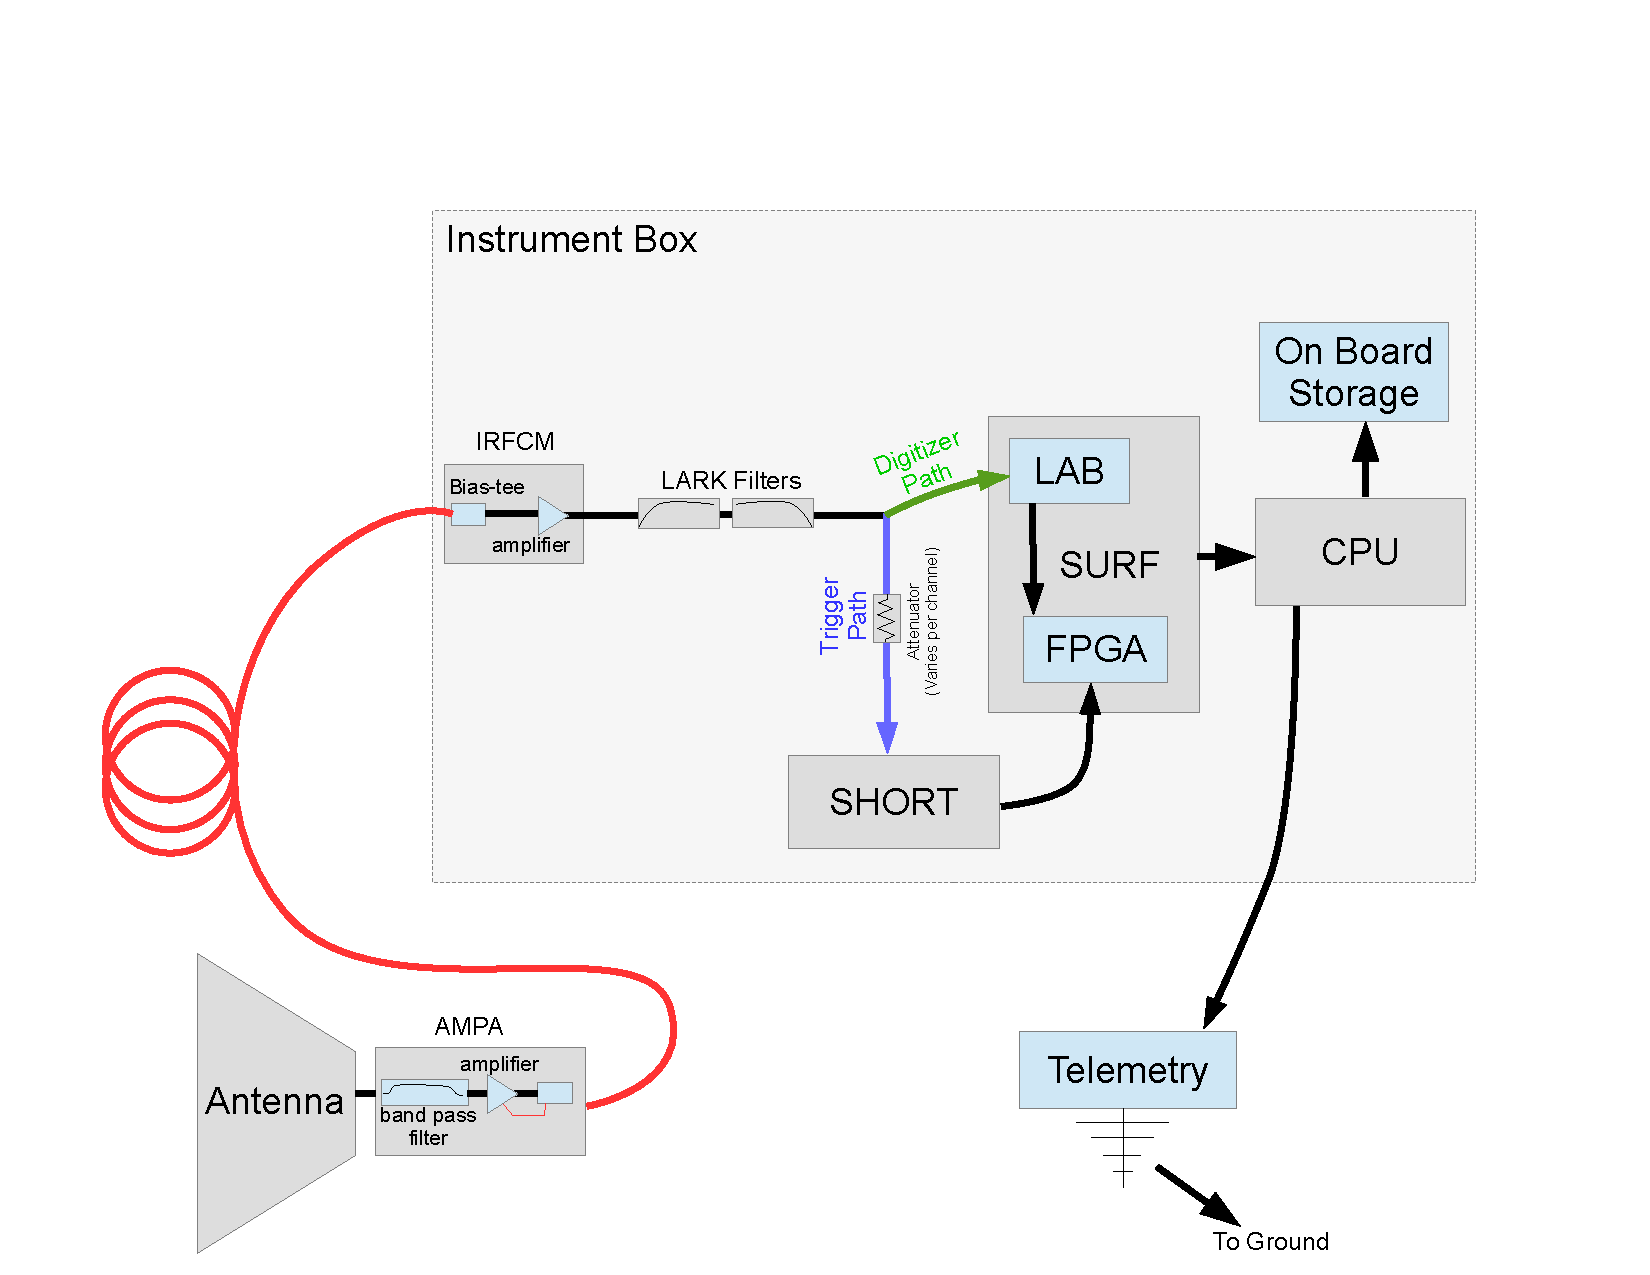
\includegraphics[width=\textwidth]{figures/RFChainBlockDiagram}
	\caption{A simplified diagram of the ANITA3 signal chain from antenna to data storage or telemetry.}
	\label{fig:RFChainBlockDiagram}
\end{figure}

	
\section{Antennas}
	The ANITA instrument's main science mission utilizes dual polarized quad ridge horn antennas to convert the electromagnetic field incident on the payload into an electrical signal that can be digitized and stored for later analysis.  The antennas design specifications include a flat gain and phase response over the full gigahertz of bandwidth, high directionality in order to reduce noise and boost signal fidelity, two orthogonal polarizations with co-located phase centers, and light weight.
	
	ANITA1 began with only two vertically separated rings and 32 antennas, however subsequent flights have packed more into the available space dictated by the flight vehicle launch envelope.  Between ANITA1 and ANITA2 an additional eight deployable nadir ring antennas were added that unfolded into flight position immediately after launch.  Between ANITA2 and ANITA3 an additional 8 antennas were added to the lower ring, equalizing the number per phi sector and bringing the total count to 48.  ANITA4, being a fast-turn-around re-flight, flew the same number of antennas as ANITA3.
	
	Antennas are located to maximize baseline distance between pairs pointing at similar regions of the field of view in order to maximize angular resolution recovered from interferometric pointing.  The benefits of increased baselines are discussed further in the calibration chapter.  The additional antennas added in each ANITA flight increase not only the number of baselines possible for this interferometric pointing, they provide an additional $\frac{1}{\sqrt{N}}$ incoherent noise reduction for coherently summed waveforms, increasing the signal to noise ratio of the final measured event.  The size of the antennas is dictated by the minimum desired frequency (f=C/$\lambda$), a term dominated by both physical payload launch envelope constraints (low frequency signals require large antennas) as well as anthropogenic CW noise, such as FM radio transmissions, in the VHF band.  
	
	The dual orthogonally facing polarization measurements from each antenna are desired to map out the complete Stokes parameters of any incident signal.  These two polarizations cause each antenna to contribute two signal channels to the total payload waveform readout array.  This measured polarization is effected by transition between air and ice at the surface of the continent.  This interaction is expected to yield an entirely vertically polarized field transient at the payload for shower interactions within the ice, and an entirely horizontally polarized transient for showers above the ice viewed via a reflection off its surface.  
	
	
	
\begin{figure}
\centering
	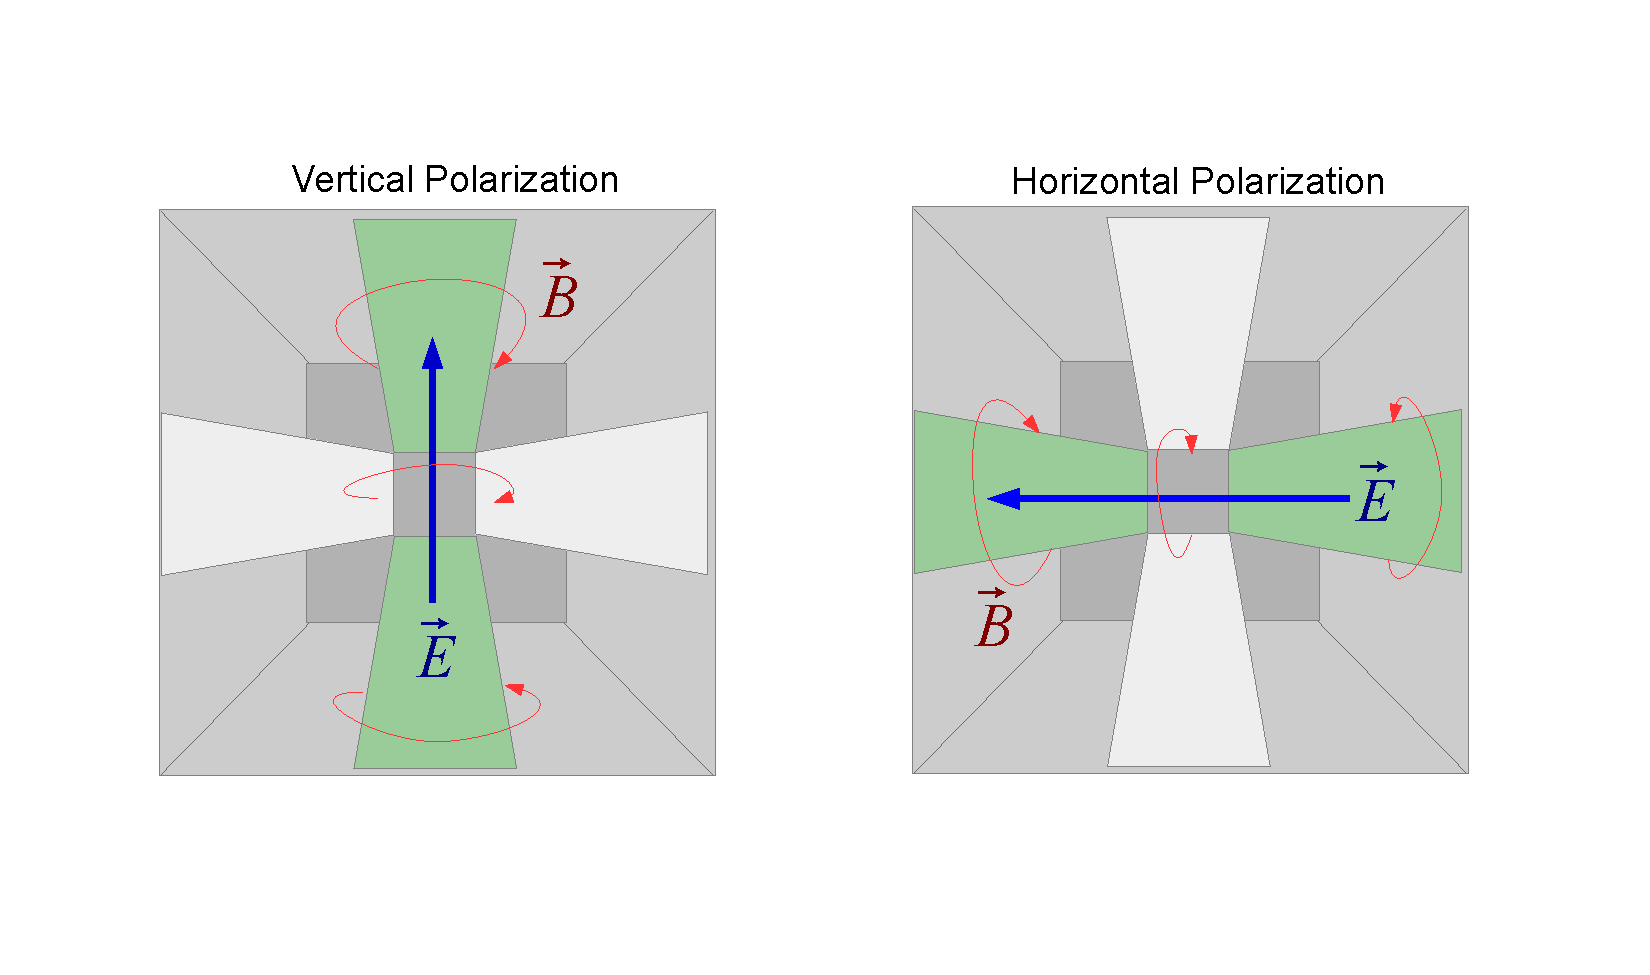
\includegraphics[width=\textwidth]{figures/AntennaPol}
	\caption{A diagram of the field line components for the Seavey dual polarization broad band horn antennas.  The E field is the principle measurement for each polarization, while the B field is the incidental cross-polarized measurement.  The antennas are specifically designed to minimize cross-polarized signal acceptance.}
	\label{fig:AntennaPol}
\end{figure}

	
	
	Calibrations of the antennas was performed over a wide range of angles in multiple configurations in order to determine the full beam-pattern of the horns in both the E-field and B-field for each polarization. See Figure \ref{fig:AntennaPol} for relation between the physical antenna and measured field orientation.  These measurements were taken for the boresight of every antenna in order to determine stability of the manufacturing process.  These measurements and variations are discussed later in the Calibration chapter.
	
%	\subsection{Antenna Theory} %seems unnecessary here?  Maybe in calibration
%		An antenna is a physical object that couples the impedance of free space to that of a a coaxial transmission wire, thus effectively converting an electric field present in a medium into a voltage that can be measured.  The principle figure of interest is in this case the antenna height, which is a mathematical construct that describes the efficiency of an antenna coupling an incident electromagnetic field into a voltage on a wire.  

	\subsection{Antenna Response Angle Justification}
		The ANITA instrument can utilize its geometric symmetry and full azimuthal coverage to reduce the response angle of the antennas and subsequently improve their signal response while keeping their noise power constant.  ANITA is very much limited by thermal background noise created from the 250K surface of the Antarctic continent, the 3K CMB, added electronic amplifier noise, and randomly placed possibly unknown anthropogenic sources.  Assuming a constant efficiency, an increase in the directivity of an antenna is linearly related to its gain by equation \ref{eqn:antGain}, where G is the antenna gain, $E_{antenna}$ is the efficiency and D is the directivity.
		
\begin{equation}
	\label{eqn:antGain}
	G = E_{antenna} * D
\end{equation}
		
		There are two maximum directivity constraints for both polarizations that each antenna must satisfy.  First, each phi sector's response must overlap with neighboring phi sector pairs to establish azimuthal directionality from interferometric baselines. Second, their elevation must encompass both up-going reflected cosmic ray and neutrino signals, as well as have some sensitivity to earth-skimming and slight down-going air showers.  As each phi sector is $22.5^{circ}$ separated from its nearest neighbor, a $30^{/circ}$ opening angle allows each sector to cover slightly over half the field of view of its neighbor.  The simple desire to have each antenna gain symmetrical in vertical and horizontal polarization then leads to a symmetric opening angle for both ridges.   Additionally, the antennas are pointed at a $10^{/circ}$ downward angle to put their maximum directivity pointed slightly below the horizon of the Earth where signals are most likely to appear.  
	
	\subsection{ANITA Low Frequency Antenna (ALFA)}
		In addition to the quad ridge horn antennas, ANITA3 flew with an additional VHF deployable "quad-slot" antenna with an omni-directional azimuthal response mounted underneath the main structure(see Figure \ref{fig:ALFA} and \ref{fig:ALFA_pic}).  As many radio frequency EAS experimental measurements are done at lower frequencies, this antenna was added to allow direct comparison between ANITA's observed particle track radiation events and those at ground based observatories.  Due to a lack of additional digitization channels in the system, as well as on-board high-pass analog filtering on the SURF board, this antenna was heterodyned with a 900MHz Local Oscillator (LO) to up-convert the signal to a measurable frequency before being combined with channel 05TH.  05TH in turn was low-pass filtered to remove it's signal and noise contribution in this signal region.  This non-symmetry in the system must be remembered in all analysis steps, and is discussed further in the Calibration section.
		
\begin{figure}
\centering
	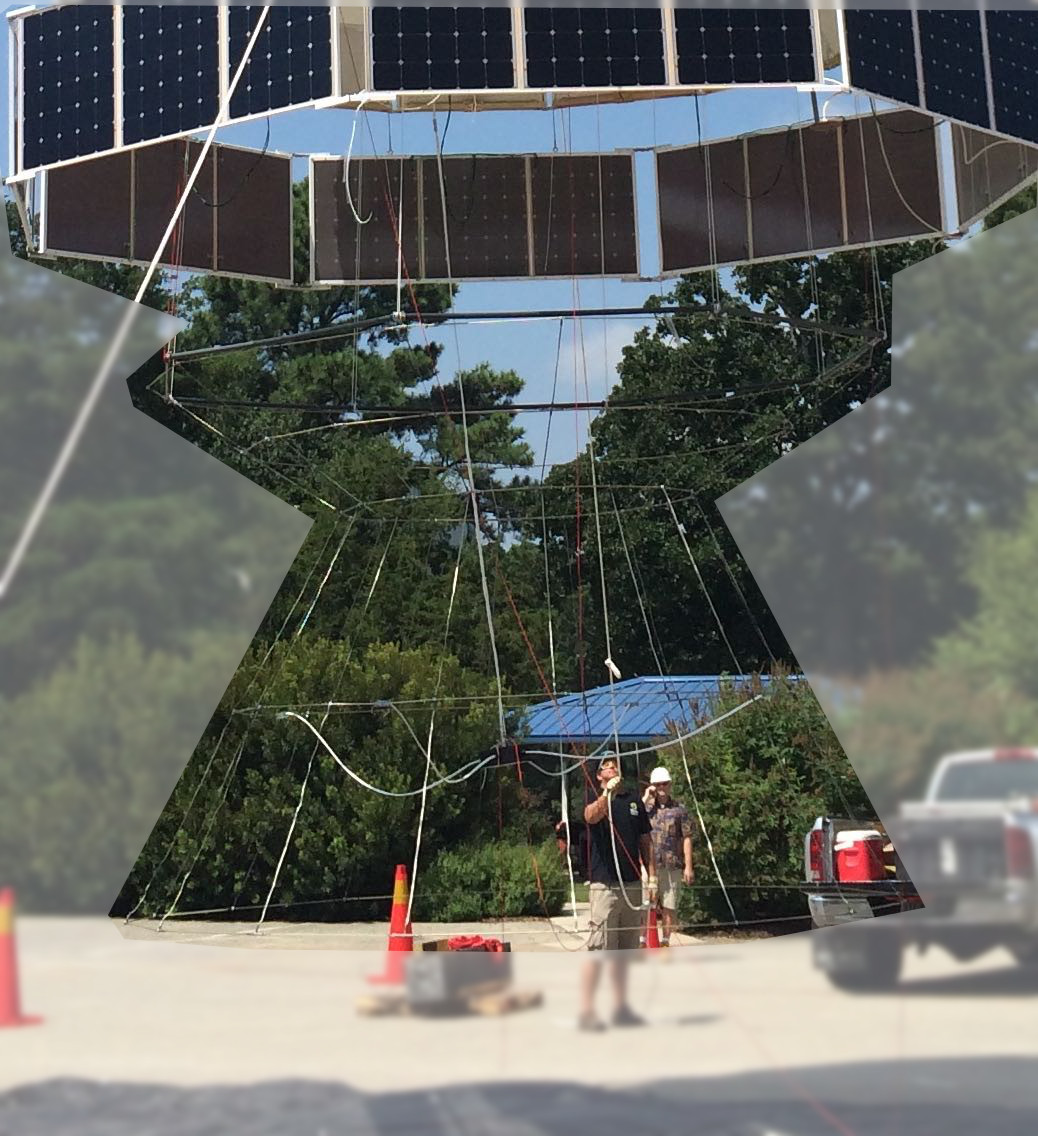
\includegraphics[width=\textwidth]{figures/ALFA_pic}
	\caption{Photo of the deployed ALFA antenna in the 2014 hang test of ANITA3 in Palestine Texas.  The photo has been edited to emphasize the outline of the antenna.}
	\label{fig:ALFA_pic}
\end{figure}

\begin{figure}
\centering
	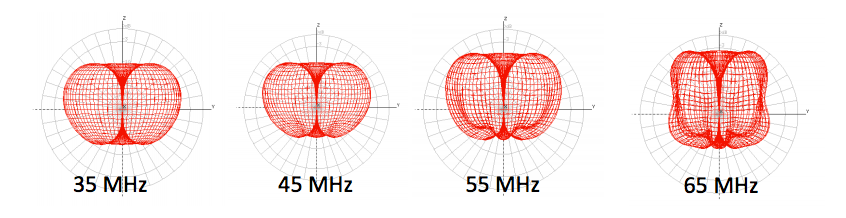
\includegraphics[width=\textwidth]{figures/ALFA_gainPattern}
	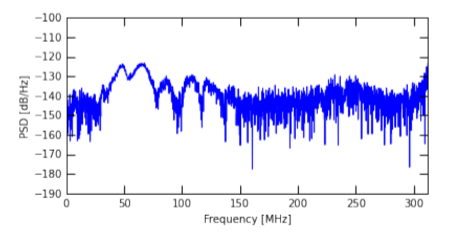
\includegraphics[width=\textwidth]{figures/ALFA_gain}
	\caption{Top: Simulations of the expected antenna gain pattern for the ALFA antenna.  Image provided by Andres Romero-Wolf.  Bottom: Measured in flight frequency response of the ALFA antenna.  Image provided by Stephanie Wissel}
	\label{fig:ALFA}
\end{figure}

	
\section{Filtering}
	\subsection{Importance}
		The radiative Askaryan and geomagnetic signal from an EAS has a very wide bandwidth, however there are a few considerations that require the signals read by the ANITA telescope be limited to a specified bandwidth.
		
		At the high frequency end of the spectrum, above 1.2GHz, the individual radiative particles in the shower core begin to be resolved, resulting in a loss of coherence of radiated power above that band (See Figure \ref{fig:AskaryanSimulation}.  This effect is stronger at angles further from the peak Cherenkov angle away from the shower axis.\cite{PhysRevD.84.103003}  This lack of coherent signal power in the UHF region provides a high frequency suppression to the total signal bandwidth.

		On the low frequency end of the spectrum, the radiated power from the shower is expected to rise as a function of frequency up to 1GHz.  Manufacturing and design limitations of a long wavelength antenna coupled with the high utilization of the VHF band by radio transmitters on satellites and ground stations lead to a requirement that lower frequencies, below 180MHz in the case of ANITA3, be removed.
		
	\subsection{Technical Details}
		This band pass filtering is done in two stages, one immediately after the antenna, before the pre-amplifier in order to prevent saturation of the pre-amplifier from out of band signals, and one after the amplification chain in order to remove out of band amplifier noise.  The primary filter must have an extremely low in-band loss, as any loss introduced by the filter is gained in full system noise temperature, a value which is cascaded through the entire amplification chain.  This was accomplished with a custom made LARK band pass filter.  The secondary filtering was accomplished with two discrete low-pass/high-pass filters that do not require such a low in band loss characteristic due to their position in the signal chain.
		
	\subsection{Digitizer Bandwidth}
		The LABRADOR digitizer also influences the selection of the band edges.  The maximum sampling rate of 2.6GS/s yields a 1.3GHz nyquist sampling frequency utilyzing .  Any out of band power will be aliased into the signal band and present itself as increased in-band noise.  Additionally, the 100ns SCA buffer length would only allow a minimum 10MHz full period oscillation to be observed.  However in reality the major limitation at lower frequencies remains to be the antennas.  The effect of the limited trigger window is visible in the ALFA low frequency antenna, as much of the 
		
\section{Amplification}
	Expected signal strength output from the coupling of the antennas to the 50-ohm RF transmission network requires that signal amplification occurs to be detectible by the available electronic instruments.  The amplification for the ANITA3 instrument was accomplished with two stages, one close to the antenna within the custom built module, and one upon entering the instrument crate itself within the iRFCM (internal radio frequency conditioning module).  
	
	\subsection{First Stage Amplifier: The AMPA and DDAMPA}
		The front end amplification was accomplished by two similar custom built modules named the Antenna Mounted Pre-Amplifier (AMPA) and the (historically named) Drop Down AMPA (DDAMPA).  Depicted in Figure \ref{fig:AMPAandDDAMPA}, each enclosure contains components for filtering, amplification, and a bias network power trasmission component.  
		
		
\begin{figure}
\centering
	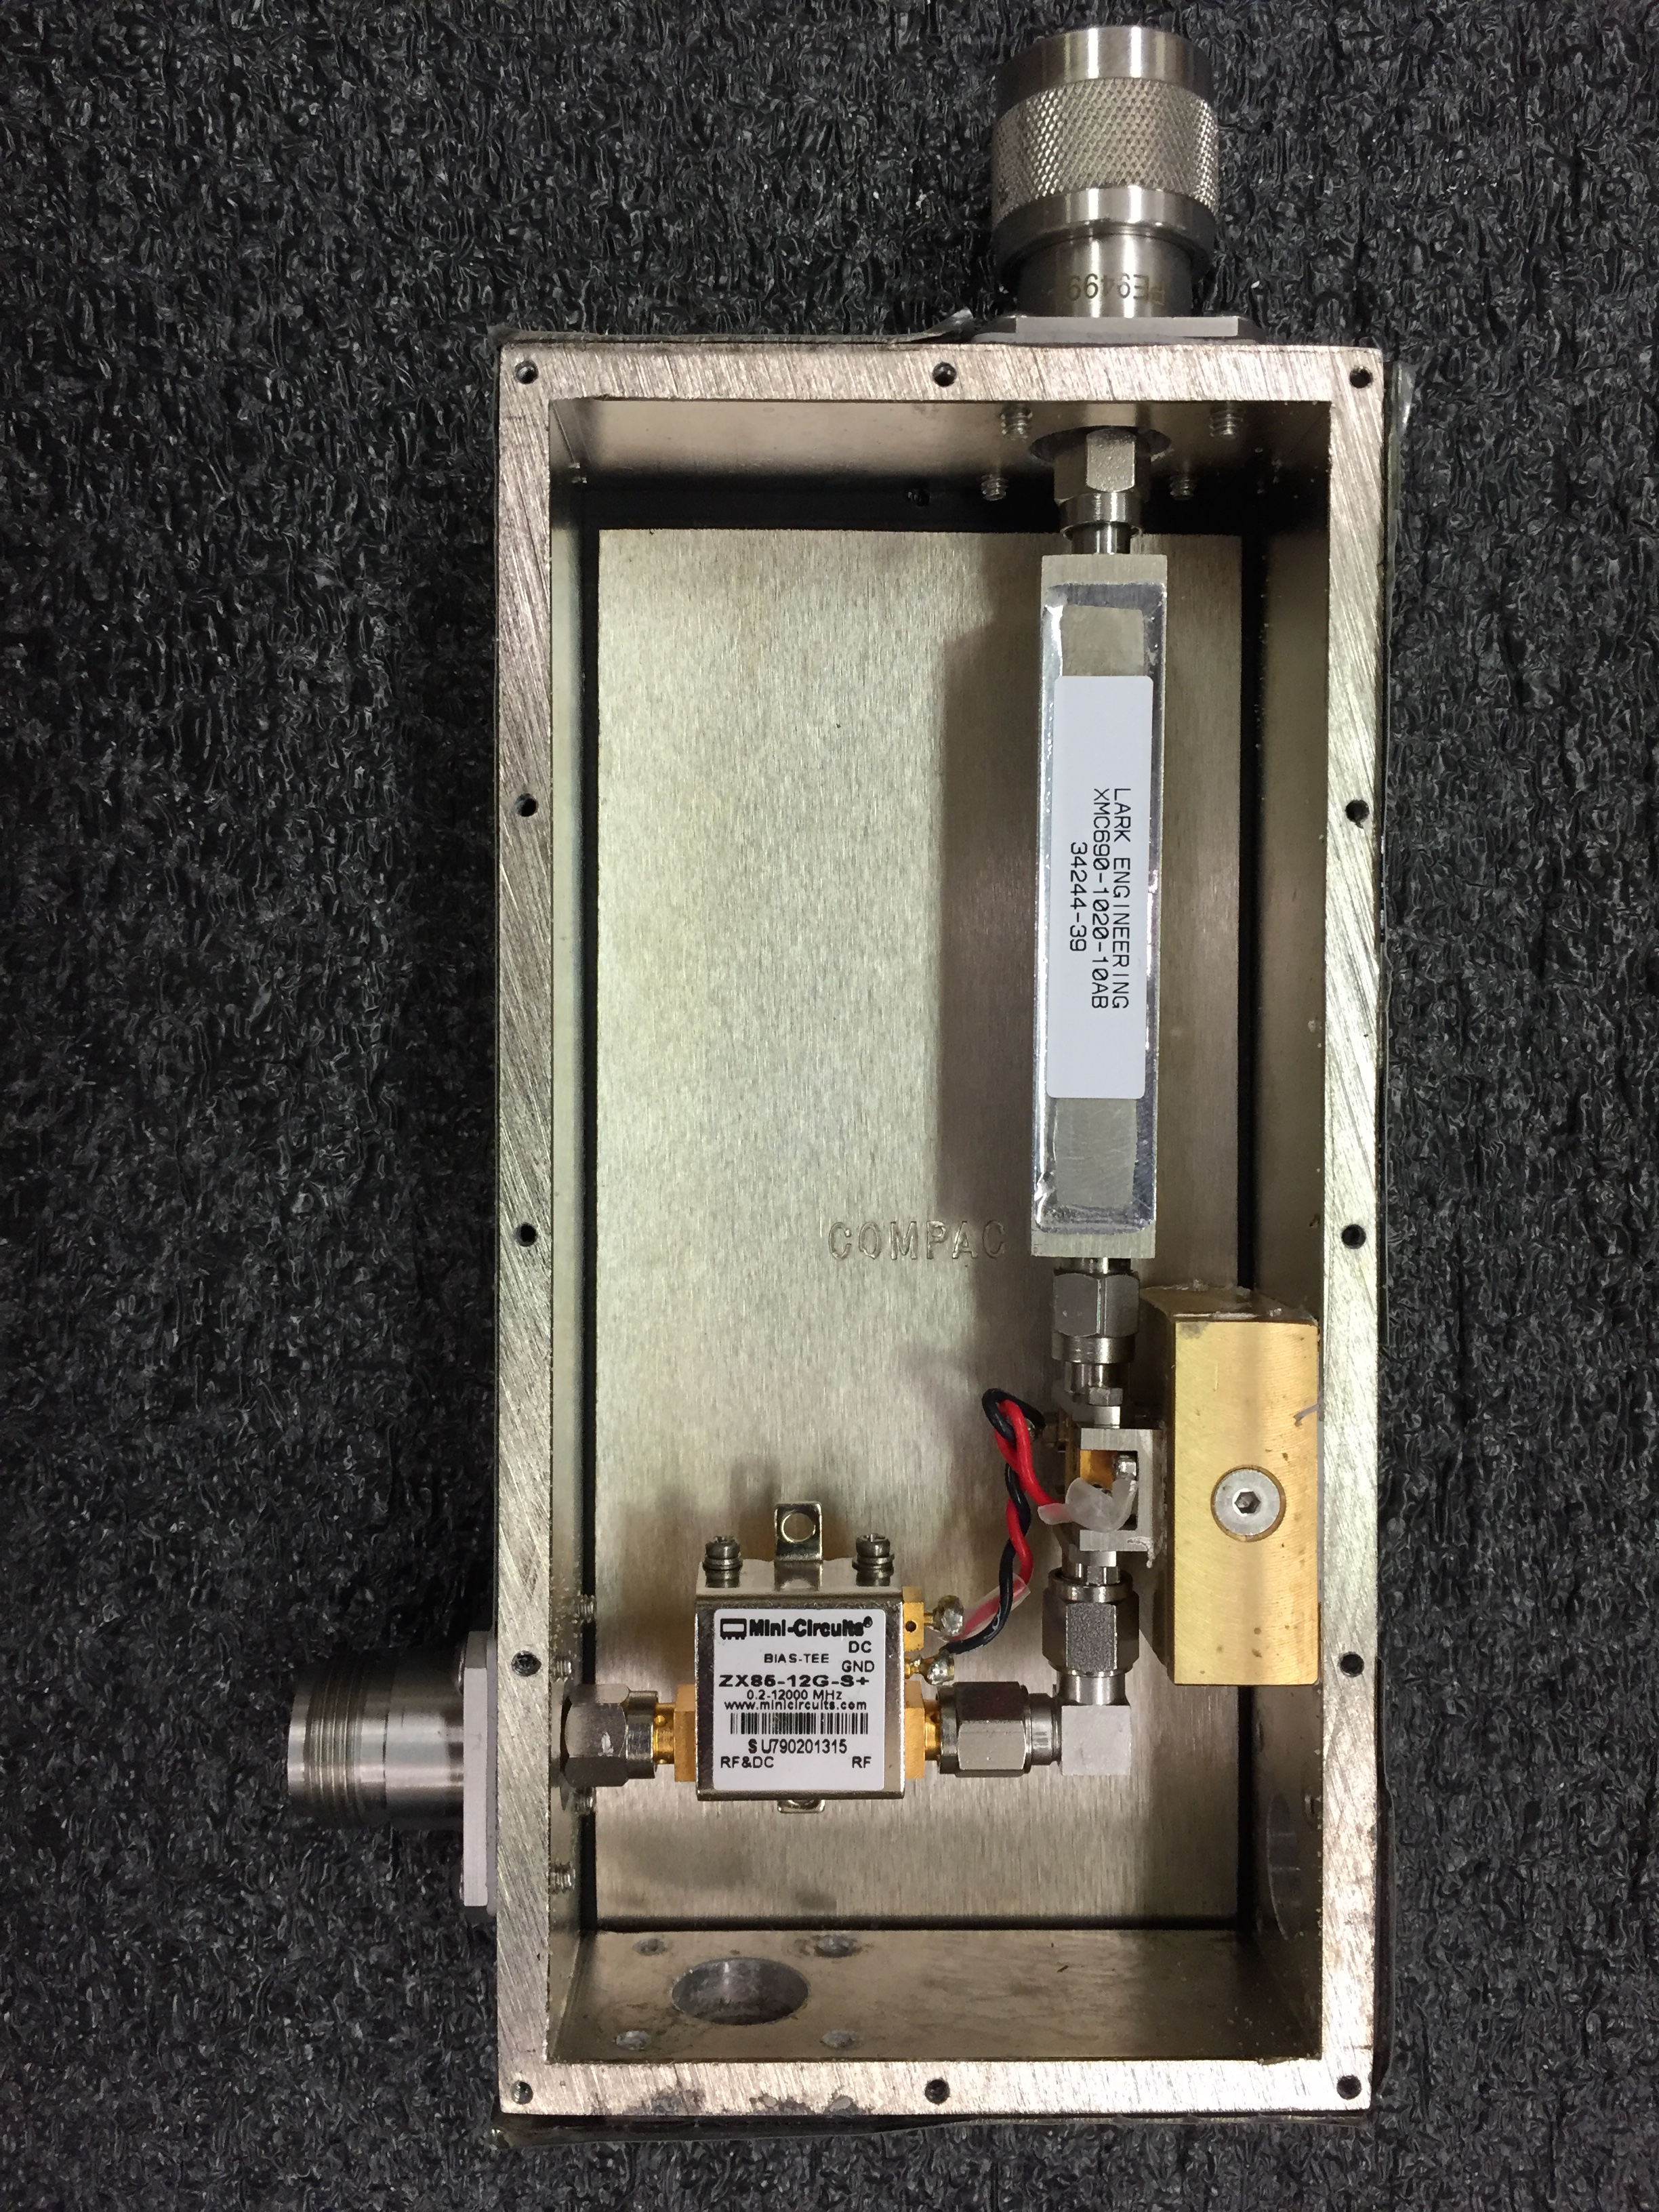
\includegraphics[width=0.45\textwidth]{figures/AMPA}
	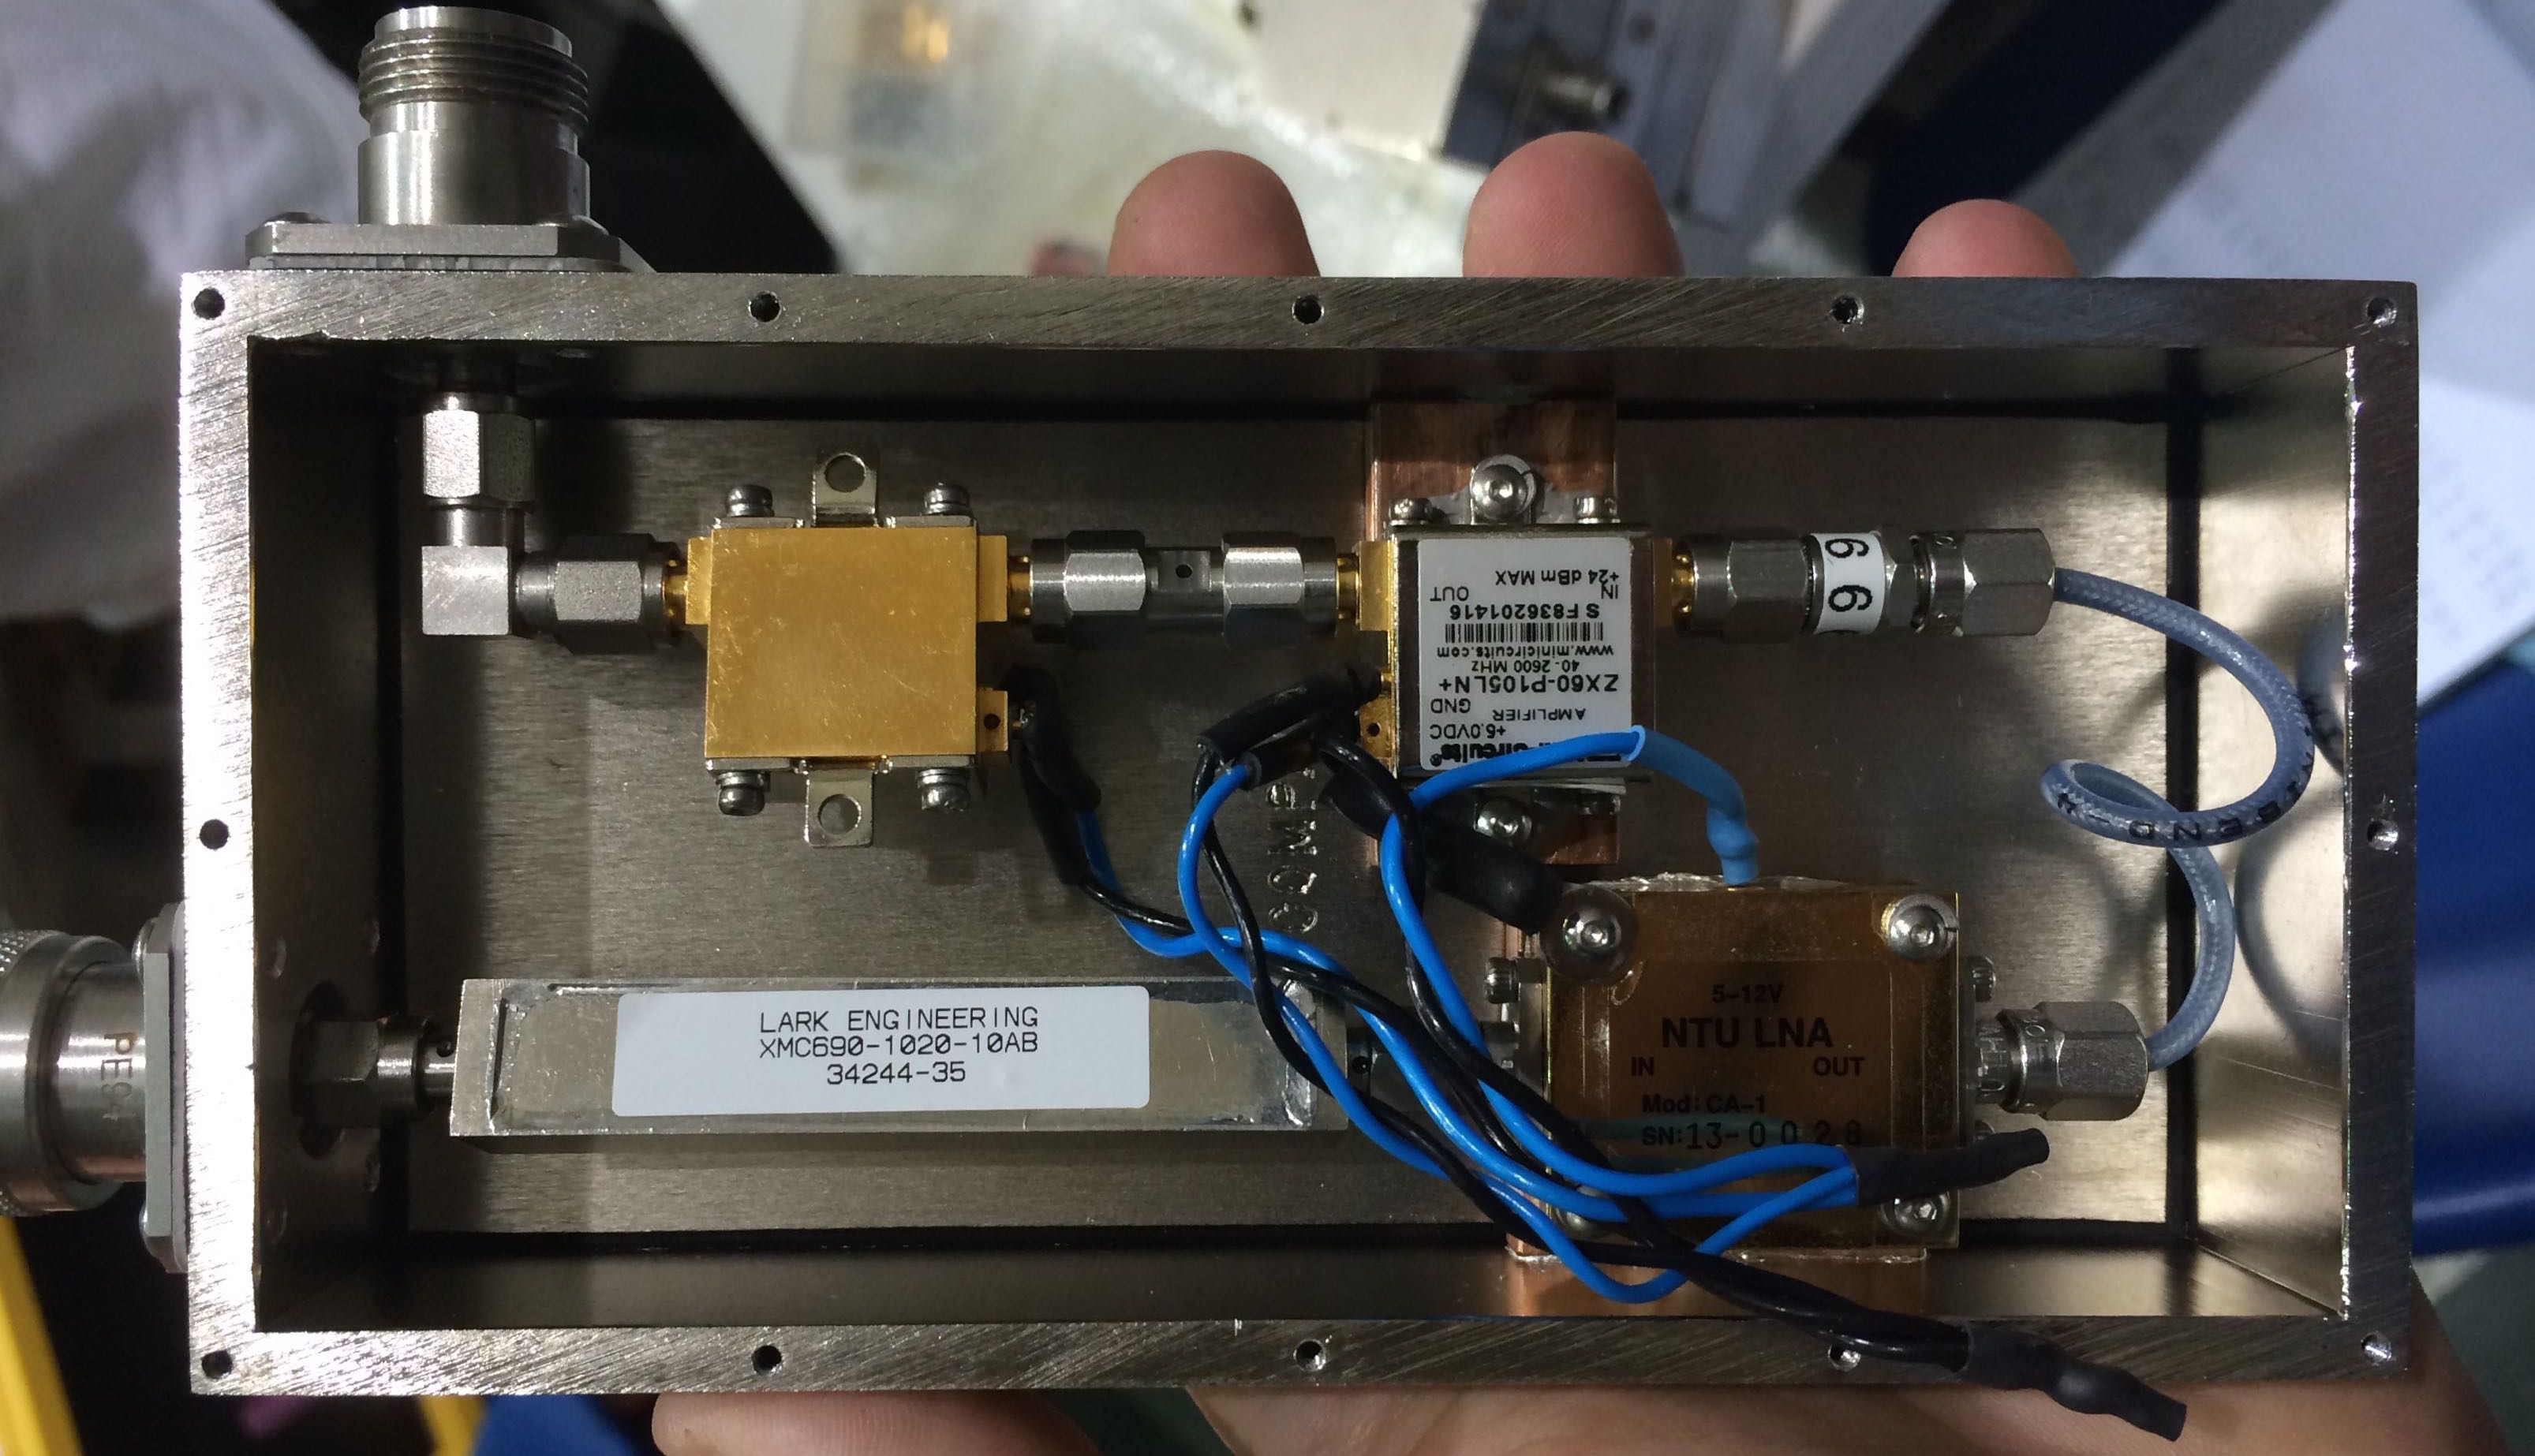
\includegraphics[width=0.45\textwidth]{figures/DDAMPA}	
	\caption{The AMPA (left) and DDAMPA (right) internals.  Thanks to Jarred Roberts for AMPA picture}
	\label{fig:AMPAandDDAMPA}
\end{figure}	

\begin{figure}
\centering
	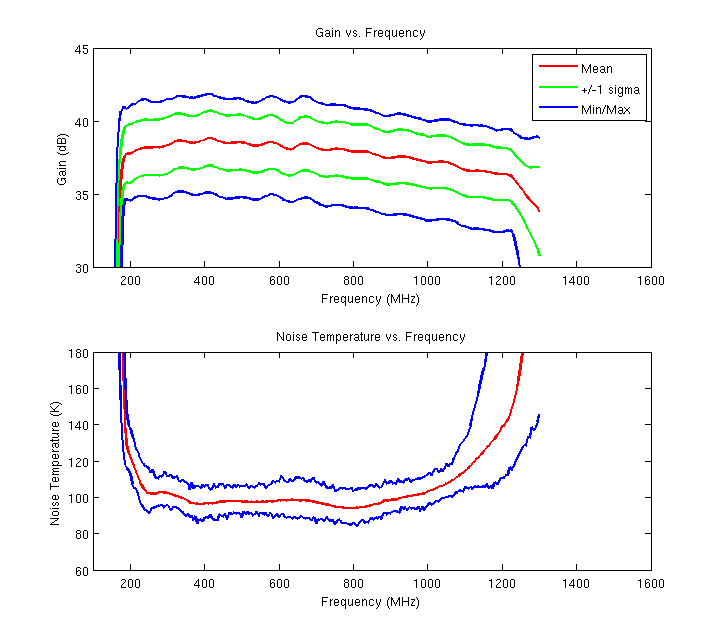
\includegraphics[height=0.45\textheight]{figures/ampas_std}
	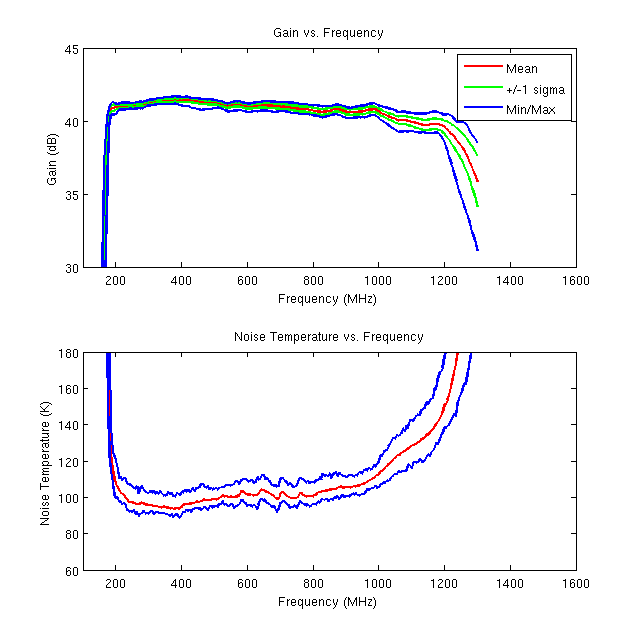
\includegraphics[height=0.45\textheight]{figures/ddampas_std}	
	\caption{Mean and standard deviation of gain and noise figure measurements for the AMPA (top) and DDAMPA (bottom) amplifier modules.  From Elog 560}
	\label{fig:AMPAandDDAMPA_std}
\end{figure}	
	
	\subsection{iRFCM}
	The four custom built iRFCM enclosures, one of which can be seen in figure \ref{fig:IRFCMpic} and is described in \ref{fig:IRFCM}, handle the second stage amplification for twenty four of the RF signal channels.  There are three major active RF components for each signal chain present within the module. The AmpLite, a high gain, high dynamic range amplifier built by Patrick Allison of OSU, a tuning attenuator for gain balancing of the 96 different channels, and a bias-tee which, as its name suggests, adds a DC bias to the center conductor of the coaxial transmission cable between the AMPA and the iRFCM.  This bias is used to power the AMPA and DDAMPA amplifier modules.

	
\begin{figure}
\centering
	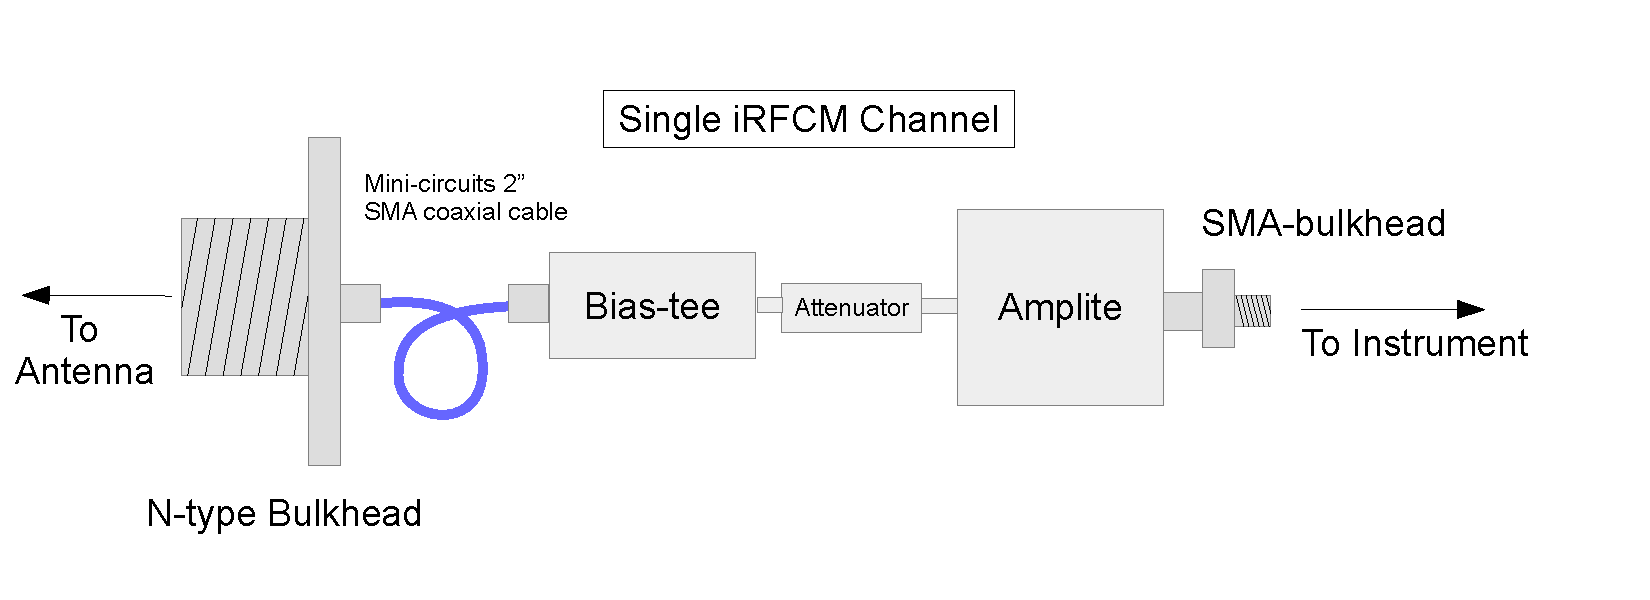
\includegraphics[width=\textwidth]{figures/IRFCM}
	\caption{A block diagram of a single iRFCM RF channel.  The bias-tee, as its name suggests, adds a DC bias to the signal }
	\label{fig:IRFCM}
\end{figure}
	
	
\begin{figure}
\centering
	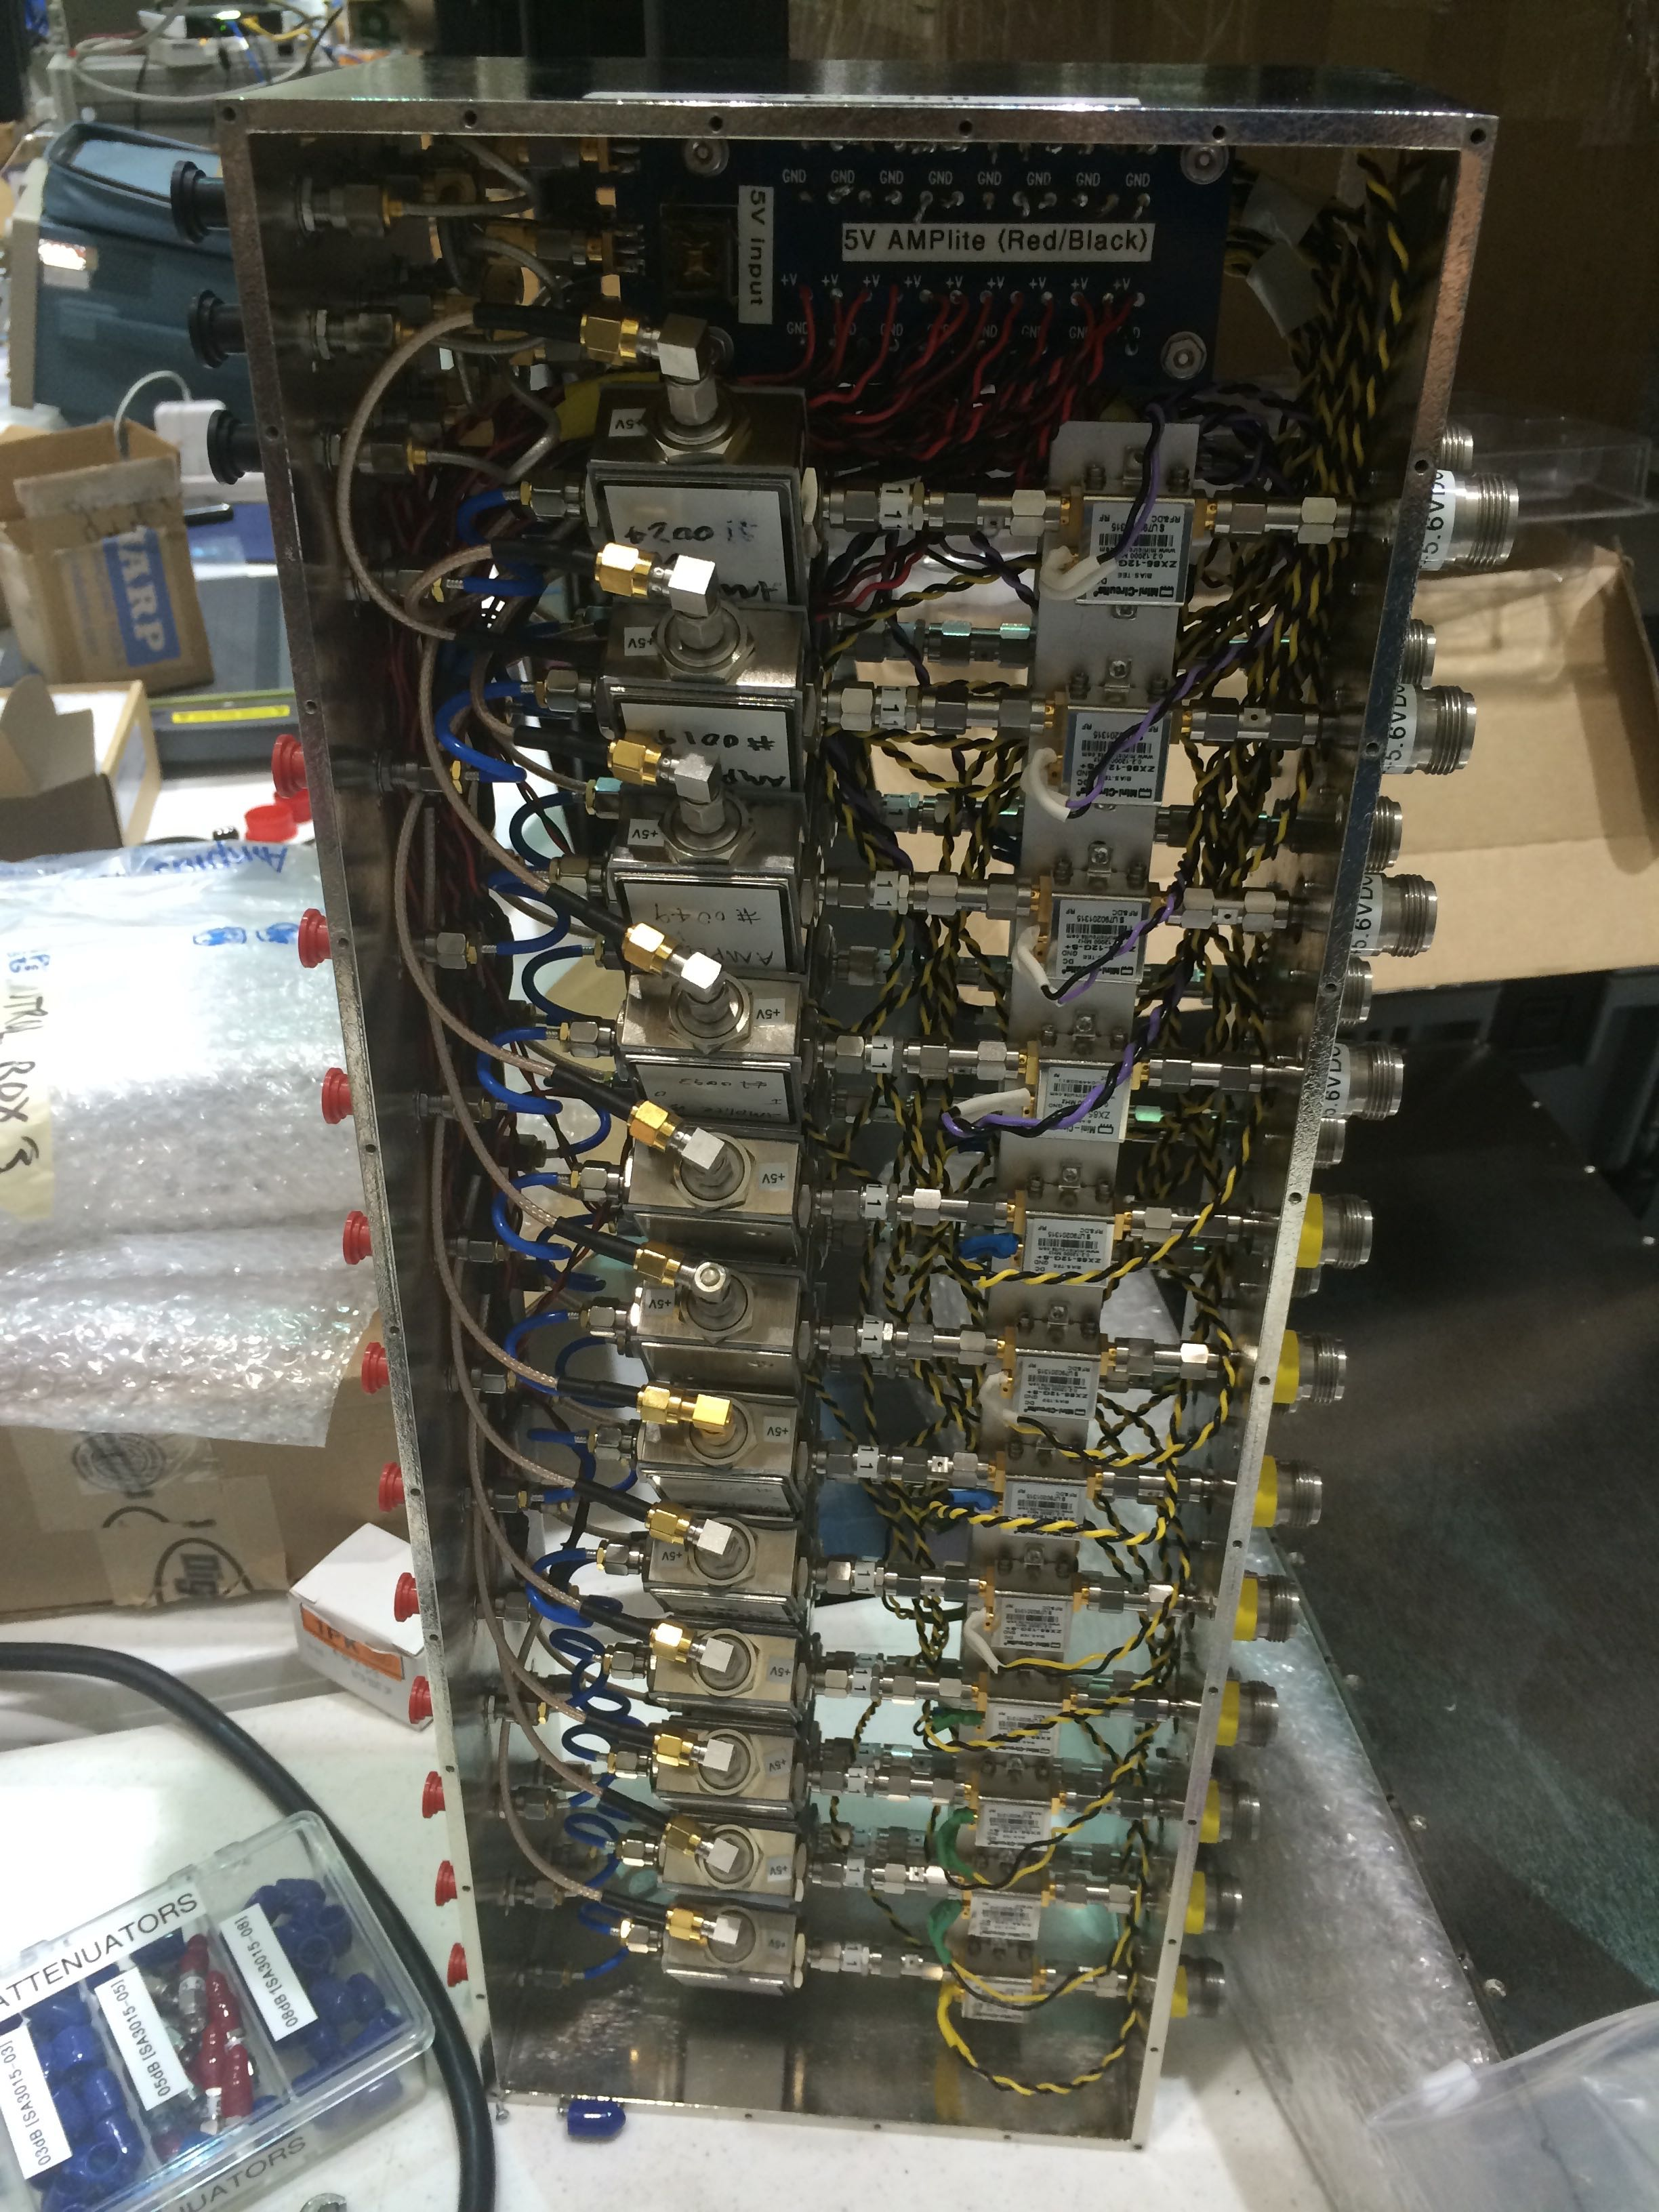
\includegraphics[height=0.9\textheight]{figures/IRFCMpic}
	\caption{An image of the internals of an iRFCM module after assembly}
	\label{fig:IRFCMpic}
\end{figure}
	
	
	\subsection{Expected electromagnetic field variations}
		Depending on the radiation mechanism being observed, the power of an EAS signal measurable at the detector is proportional to the energy of the incident cosmic ray particle.\cite{EASSignalPower}  This signal power is superimposed on the thermal and anthropogenic background noise present in the field of view of the detector.  The constant thermal emission of matter in the field of view of an antenna introduces a Johnson-Nyquist thermal noise component, which is calculated in Equation \ref{eqn:NyquistNoise}

\begin{equation}
	\label{eqn:NyquistNoise}
	P = k_{b}T\delta F
\end{equation}

Where P is the thermal noise power observed across a termination resistor in watts, $k_{b}$ is Boltzmanns constant, T is the absolute temperature observed temperature in kelvin, and $\delta F$ is the frequency bandwidth in Hz.  The antenna, creating a smooth transition between the complex impedance of free space and that of the coaxial transmission network, has a noise temperature dictated by the integral of the temperature of objects in its field of view $(T(\theta,\phi))$, weighted by the gain pattern of the antenna $(G(\theta,\phi,\omega))$, shown in equation \ref{eqn:antTemp}.

\begin{equation}
	\label{eqn:antTemp}
	\int_{-\pi}^{\pi}\int_{\theta}^{2\pi}\int_{0}^{\infty} G(\theta,\phi,\omega)*T(\theta,\phi)sin^{2}\theta d\theta d\phi d\omega
\end{equation}


	\subsection{Noise Figure} 
	The requirement of amplifier chains leads to a minimum of additional electronics noise introduced by the detector.  Besides a background of thermal noise, the dominant continuous noise source is electronics noise from the amplifiers.  This noise is a byproduct of the non-ideal coupling of the amplifier to the input signal that results in the amplification of internal thermal noise seen as a resistance on the front of the amplifier.   This noise, unlike the thermal noise incident on co-pointing antennas, is not coherent as each amplifier adds its own uncorrelated noise component.  The noise figure is additionally increased by any loss of power in front of the amplifiers.  Since the noise figure cascades through an amplifier chain, it is imperative to reduce any additional noise figure at the beginning of the signal chain, and less important in the subsequent amplifiers.  The cascading noise can be calculated using Frii's Formula (Equation \ref{eqn:noiseCascade}), where $T_{total}$ is the resulting noise temperature of the entire signal chain, $T_{n}$ is the noise temperature of a specific element, and $G_{n}$ is the gain magnitude of a specific element.
	
\begin{equation}
	\label{eqn:noiseCascade}
	T_{total} = T_{1} + \frac{T_{2}}{G_{1}} + \frac{T_{3}}{G_{1}G_{2}} + ... + \frac{T_{n}}{G_{1}G_{2}...G_{n-1}}
\end{equation}
	
	From this, one can see that the +38dB of gain from the first stage amplifier reduces any subsequent noise figure from components by a factor of $38dB = 10*log(G) \rightarrow 10^{38/10} =  6309 = G$. alleviating the requirement for low noise amplifiers in subsequent stages.


	\subsection{Dynamic Range}
		The absolute power level of the signal travelling through the system is dependent on the end-of-chain termination and instrumental device, and must be tuned appropriately.  For example, the digitizer ASIC can cover a 2.5V full dynamic range.  An observed voltage with peak amplitude significantly below that level would never exercise the range boundaries of the digitizer.  A negative drawback to this wasted range is that the lesser significance bits lose sensitivity to low voltage oscillations, as fewer total levels fully encompass the full signal.  Equally and oppositely, too high an input power signal would become distorted at high peak amplitudes. Other systems at termination ends of the branching signal chain have similar dynamic range limitations and must be tuned appropriately.
		
		
	\subsection{Gain Justification}
		The required gain of the system can be arrived at by determining the maximum terminal instrumentation requirement input power, then calculating what additional amplification is required to meet that specification.  Any terminal instruments that require lower input power are achieved by in-line, flat spectrum, fixed attenuator components.  \ref{tab:rfLinkBudget} is a table of the terminal components, their dynamic ranges, and the required gain necessary to put observed thermal noise from the antenna into a measurable power region.  Components not yet mentioned in this thesis are covered in subsequent sections in this chapter.
	
\begin{figure}
	\centering
	\label{tab:rfLinkBudget}
	\begin{tabular}{| l | c | c |}
		\hline
		Component & Dynamic Range & Gain Requirement\\
		\hline
		LABRADOR digitizer & 20dBm & 80dB \\
		RF Power Monitor & -10dBm & 50dB \\
		SHORT Tunnel Diode & 0dBm & 60dB \\
		\hline
	\end{tabular}
	\caption{A description of the required input power and gain requirements for the three terminal instrumentation components of the ANITA3 system}
\end{figure}
	
	
\section{Digitization}
	The electric field variations incident as a function of time is digitized using an array of fast analog to digital converters (ADCs), custom designed application specific integrated circuits (ASICs).  The ANITA3 instrument utilizes a LABRADOR (Large Analog Bandwidth Recorded And Digital Ordered Readout) chip, designed by Gary Varner.  It is a 12-bit, 2.4GS/s, 256 sample long ADC, yielding a window size of ~100ns.  This is accomplished with a sample and hold ring buffer read out with a wilkinson clock comparing the stored charge in a storage capacitor against a ramp signal driven by a constant current source.  Each chip receives 8 RF analog inputs, as well as a 9th clock channel coincidently propagated to all LAB chips.  The SURF (Signal Unit for Radio Frequency) Board consists of 4 LABRADOR chips in order to create a buffer for continuous sampling.  

	\subsection{LABRADOR3 ASIC}
		The third iteration of the Large Analog Bandwidth Recorder And Digitizer with Ordered Readout (LABRADOR, or LAB3) has been in use on ANITA flights due to its extremely low power and high precision.  It consists of a nine RF channels fed into separate 260 cell capacitor ring buffer and can operate at sampling frequencies of 2.6GS/s, or a Nyquist limit of 1.3GHz.  In addition, it has a large dynamic range and a gigahertz of bandwidth in the UHF spectrum.  The sampling time base is driven by a phase inverting Ripple Carry Out pulse that propagates internally to the chip.  The continuous sampling is halted when a trigger is issued to the chip, and a Wilkinson Clock measuring the Time To Threshold of a constant current ramp voltage converts the stored charge in each capacitor to a digital value that is read out in parallel to an FPGA for storage.  Due to the dead time related to the digitization process, four LAB3 chips are placed in parallel in order to ensure continuous sampling even when a single LAB3 is reading out its values.  When a hold is issued, the LAB3 chip returns both an estimate of which RCO phase it is in (which is incorrect near the wraparound region), as well as the locations of the "HitBus", or samples that are currently connected to the RF input. The procedure and results of calibrating this readout is detailed in the Calibration section.
		
\begin{figure}
\centering
	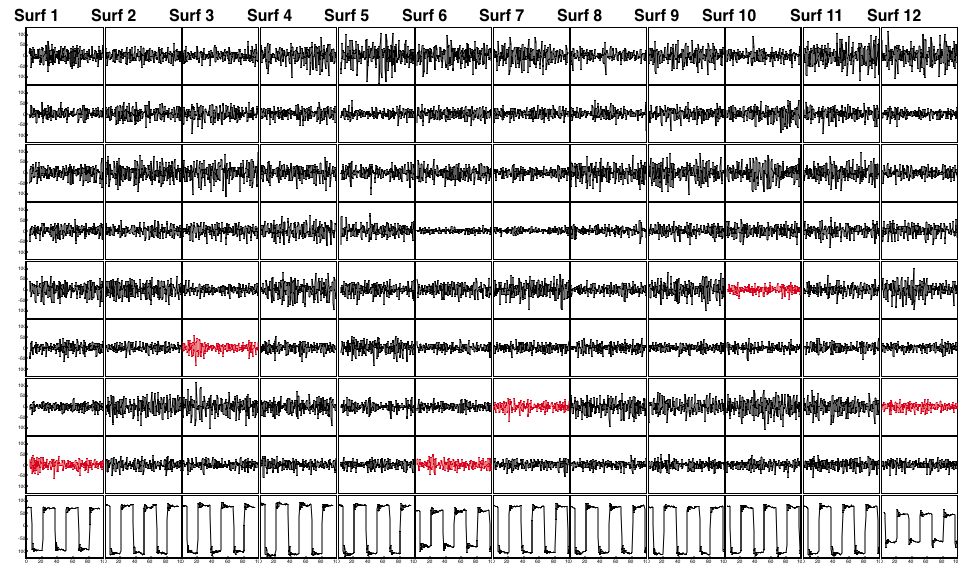
\includegraphics[width=\textwidth]{figures/waveformSnapshot}
	\caption{An example readout of all 96 channels of the full ANITA3 detector, organized by SURF (columns) and channels (rows).  Bottom row is the synchronization clock inserted into all LAB chips.  In red are phi sectors that triggered the event.  This particular waveform is low SNR self triggered WAIS calibration pulser (ev 61326092).  Image made with MagicDisplay data visualization code.}
	\label{fig:waveformSnapshot}
\end{figure}
		
	
	
	\subsection{Limitations}
	After a hold is issued to a chip, the digitization freezes the ring buffer and yields the chip unable to sample until readout is complete, a process that can take ~1us.  During a readout, no new data can be captured by the LABRADOR chip.  To alleviate this, the RF input chain is separated into four separate chips which are read out one at a time.  This provides a buffer depth of four which allows the instrument to remain live even while reading out several repetitive events.
	
	The analog bandwidth of the LAB3B (used in the ANITA3 and ANITA2 experiments) did not fully cover the full bandwidth of the antennas and signal chain due to coupling into the chip through the bond wires in the package.  This yields a drop-off in sensitivity to high frequency signals.  
	
	The time between samples is controlled by a charge starved transistor chain that controls the connection between the sampling capacitor and the input RF signal.  Due to process inconsistencies in the manufacturing of the ASICs, the timing between subsequent samples is not well controlled.  This yields a variable delta T that needs to be corrected in calibration of each chip individually.  In addition, it leads to an unevenly sampled time domain waveform, which introduces a difficult to correct frequency response, and requires interpolation between points before creating interferometric maps.  This is processing intensive, an issue that makes doing on board interferometry more difficult.
	
 	Since each LAB chip can only digitize eight channels concurrently, a total of twelve total SURF boards are required to read out any particular event simultaneously.  The dispersal of the readout HOLD signal from the FPGA, and its subsequent latching on each LAB, adds jitter that needs to be corrected out.  The ninth channel on each lab observes a 33.3MHz analog clock signal propagated through the CPCI backplane to each SURF.  By measuring the relative phase of this clock between SURFs, a correction for this jitter can be done.  This is discussed further in the Calibration section.
	
	\subsection{Impulse Response}
	The filtering and amplification chain has a dispersive effect on the signal, which requires a calibration of the system impulse response in order to fully understand the incident electromagnetic field.  An impulse response is the phase and gain distortion created by the RF network to an input signal.  In the ANITA system, an band limited case, the phase shift increases as a function of frequency, which causes the signal power to be temporally spread.  As a cross-correlation between multiple channels is dependent on the full complex parameters of the signal, significant variation between the impulse responses of channels will result in a reduced maximum correlation value regardless of the electromagnetic impulse present at the antennas.  The ANITA instrument is designed to be identical and symmetrical across all 96 channels, making this effect small and constant.  Measurements of this response and calibration are done in the Calibration section, and the effect and deconvolution is detailed in the Analysis section.

	
	\subsection{Future development}
	Since the LAB3B was developed in 2005, there has been significant development in the LABRADOR architecture.  The most modern generation of chip, the LAB4D, is a single channel readout that improves upon the previous generations by both vastly increasing the storage buffer through use of a Storage Capacitor Array (SCA) to increase the record length or buffer depth of the chip.  It also allows for the correction of dT offsets iteratively onboard the chip, minimizing the requirement for post-digitization correction of the waveform and the subsequent high-frequency signal loss.  The quantitative effects created from a large dT variance are discussed later in this thesis.
	
		
\section{Triggering}
	As the time domain digitization window is extremely small (100ns is one ten millionth (1e-7) of a second) and ANITA is limited to a 50Hz readout rate, it is necessary to selectively trigger on segments of time that have a high probability of containing a signal event.  The physics signal created by a UHE particle interaction within the field of view of, and directed towards, the instrument exhibits itself as a picosecond duration impulsive electrical potential emanating from a specific direction.  The background is random incoherent thermal noise or single band constant power anthropogenic sources.  As there is no digitizer buffering or analog delay lines, the triggering system must combine together information from several RF channels without full digitization and form a decision quickly, before the waveform is overwritten in the ring buffer of the LABRADOR digitizer.  For the ANITA3 system, these triggering decisions were made in the Triggering Unit for Radio Frequency (TURF), which receives trigger information for each channel from FPGA comparator electronics on each SURF through the CPCI backplane passthrough connectors.
	
	\subsection{SHORT square-law power integrator}
		A solution to triggering employed in many RF transient detector experiments is to utilize a square-law integrating power detector.  An Ezaki diode (or tunnel diode), is a nonlinear semiconductor circuit that, in a specific input power region, essentially rectifies and integrates an incoming RF signal through the quantum mechanical effect of electron tunneling.  The diode is capable of taking the extremely fast impulsive signal, with a pulse width of under 1ns, and distributes the power over a longer time scale while simultaneously increasing the signal to noise power ratio.  This allows a clocked comparator circuit, usually running with a max of 4ns/cycle, to latch a electrical signal that crosses a certain threshold.  These L1 triggers can be tuned to a reasonable rate, the specifics of which is detailed below, by altering the comparison voltage with an on board DAC, and each channel can be kept running at a similar rate with a PID loop.  Comparing the timing of these "L1" triggers between antennas with similar pointing directions allows a massive decrease in overall trigger rate dictated by combinatorics.
		
\begin{figure}
	\centering
	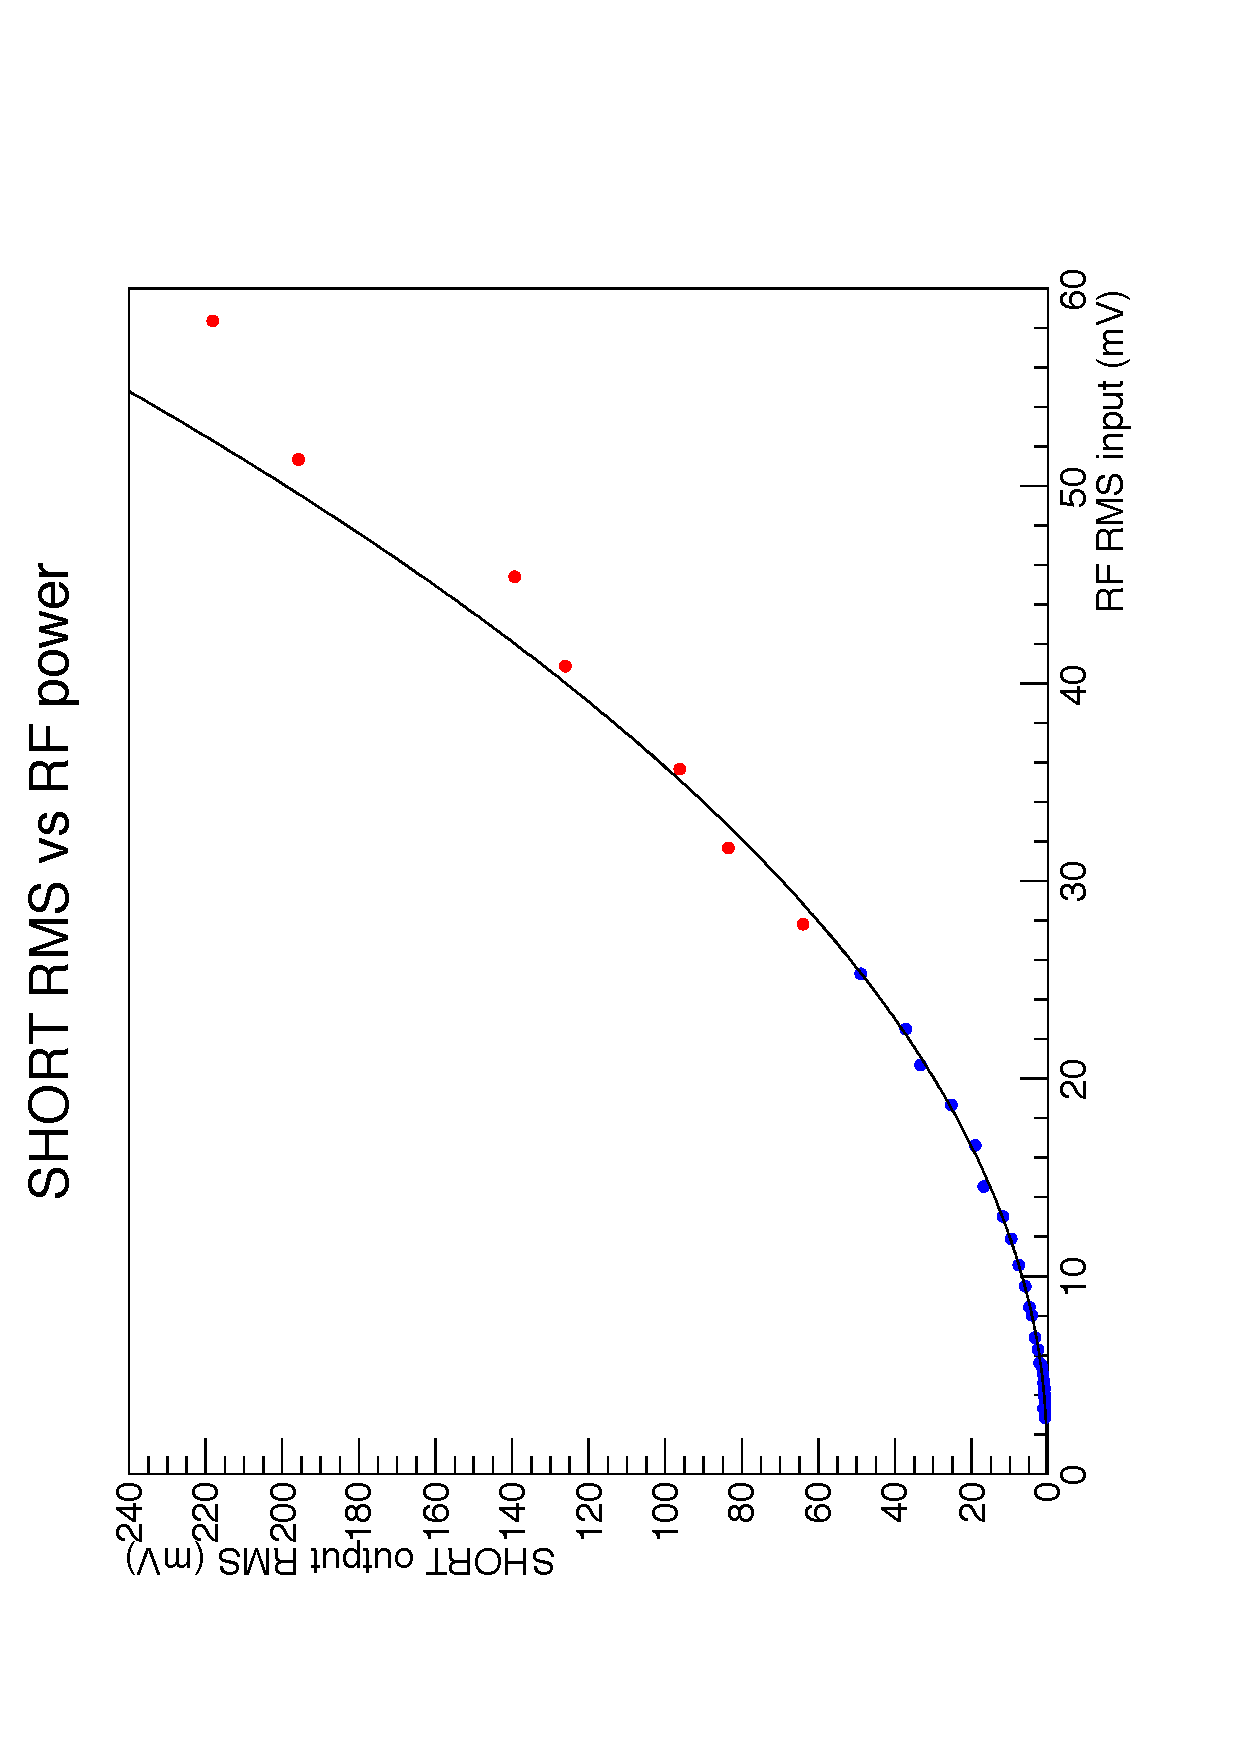
\includegraphics[height=0.8\textheight,angle=-90]{figures/RMS_in_out}
	\caption{Measurements of the response of the SHORT tunnel diode "square law" RF power detector taken in Palestine TX in 2014.  Thanks to Katie Mulrey for the plot}
	\label{fig:SHORT_square}
\end{figure}
		
	
	\subsection{Trigger Heirarchy Overview}
		The triggering system is divided into several sub-triggers that layer hierarchically to arrive at a global trigger decision.   These range from the individual power law thresholding to a time windowed combinatoric trigger between multiple channels.  In ANITA3, the trigger is split into a vertical (Vpol) and Horizontal (Hpol) trigger system, as the two differing particle shower sources (in ice neutrino interactions vs geomagnetically dominated air showers) will have mostly orthogonal polarization.  These two trigger paths are identical and have equal weighting in the final global trigger decision.  
		
		The first trigger level, or what I'll call the L0 trigger (it is also known as the L1 trigger depending at what value one begins counting), is a comparator circuit on the FPGA between the output of the SHORT and a tunable DAC. It is thus possible to tune each channel individually to give an even weighting in the ultimate trigger decision.  This is done by measuring the number of threshold crossing counts per time fraction observed by each comparator circuit, also called the scalar rate.  This scalar rate is monitored by a software PID servo loop that attempts to keep all channels equal.
		
		The secondary trigger level, or L1, is a phi sector specific time dependent windowing function that combines the L0 triggers from all three channels in a single phi sector.  A real plane wave signal incident on a phi sector will have a causal separation in time, while incidental noise threshold crossings will be uncorrelated in time.  These timing offsets are used to create a metric for discriminating on noise up to the level of precision provided by the FPGA trigger electronics.  
		
		The final trigger, or L2 is a requirement that two neighboring phi sectors decide a L1 trigger within an 8ns window.  This leads to the ultimate requirement that four out of six like-polarized antenna channels with an overlapping field of view observe a transient power fluctuation.  Additional details of each level trigger are detailed below.
		

	\subsection{L0 Tiggering efficiency and quality}
		The trigger must make a trade off between efficiency, the ratio of real signals selected for digitization over the total number of signals incident on the detector, and quality, the ratio of the number of true signal event over total selected events.  A perfect detector would have an efficiency of 1 and a quality of 1.  However in reality these values are both a function of the total maximum readout rate for the detector, which places a maximum limit on the number of events capable of being selected.  As an example, if the trigger constantly selected all moments in time it would be perfectly efficient, but the quality of the signal would be horrific.  Inversely, if the trigger was set to have perfect quality and only select extremely high power impulsive events, it would have poor efficiency for low SNR signals.  The efficiency of the detector can be statistically measured by injecting signals of varying signal to noise ratio (SNR) at a known rate and observing the rate of measured signals.  This will produce a curve (as seen in a plot I will add) which has a characteristic shape, of which the 50\% efficiency point is the defining metric.  This point will be directly related to the allowable incidental noise trigger rate, which was decided to be set at a rate where the payload would be "dead" for approximately 5\% of the time.  I have to add plots for these things!
		
	\subsection{L0 Optimization}
		What little room lies in optimizing the SHORT circuit is entirely in tuning the input power to the tunnel diode circuit.  The inverse-resistance region, where a decrease in voltage yields an increase in current flow, is the primary region where additional input power yields an output that is a square of the input.  This occurs at an extremely low power level, much below the minimum quantization level of the LABRADOR ADC, and thus the power must be attenuated in the signal chain after the split between the trigger and digitizer paths.  In addition, the output power of a fully optimized tunnel diode circuit is extremely small,	requiring amplification to produce a working range for the comparator circuit commensurate to the output of a DAC.  The resolution ( (trig rate)/(DAC count) ) dictates the stability of the trigger system.  If this value is too high, changing the trigger threshold setting for a specific channel would cause a large jump in the overall trigger rate of the system, and possibly allow a channel to dominate (or be excluded from) the global triggers.
		
		
	\subsection{L1 Pseudo-Pattern Trigger}
		The L1 trigger consists of a time windowed and multiple antenna combinatoric selection.  As a real signal pulse will have a correlated plane wave that passes across the physical locations of each antenna, a time coincidence of the signal is required.  This helps to reduce thermal noise triggers, which will be uncorrelated to the locations of the antennas.  In addition, this allows us to use the narrow opening angle of the antennas and their high gain to make a rough directional cut on the incoming signal.
		
\begin{figure}
	\centering
	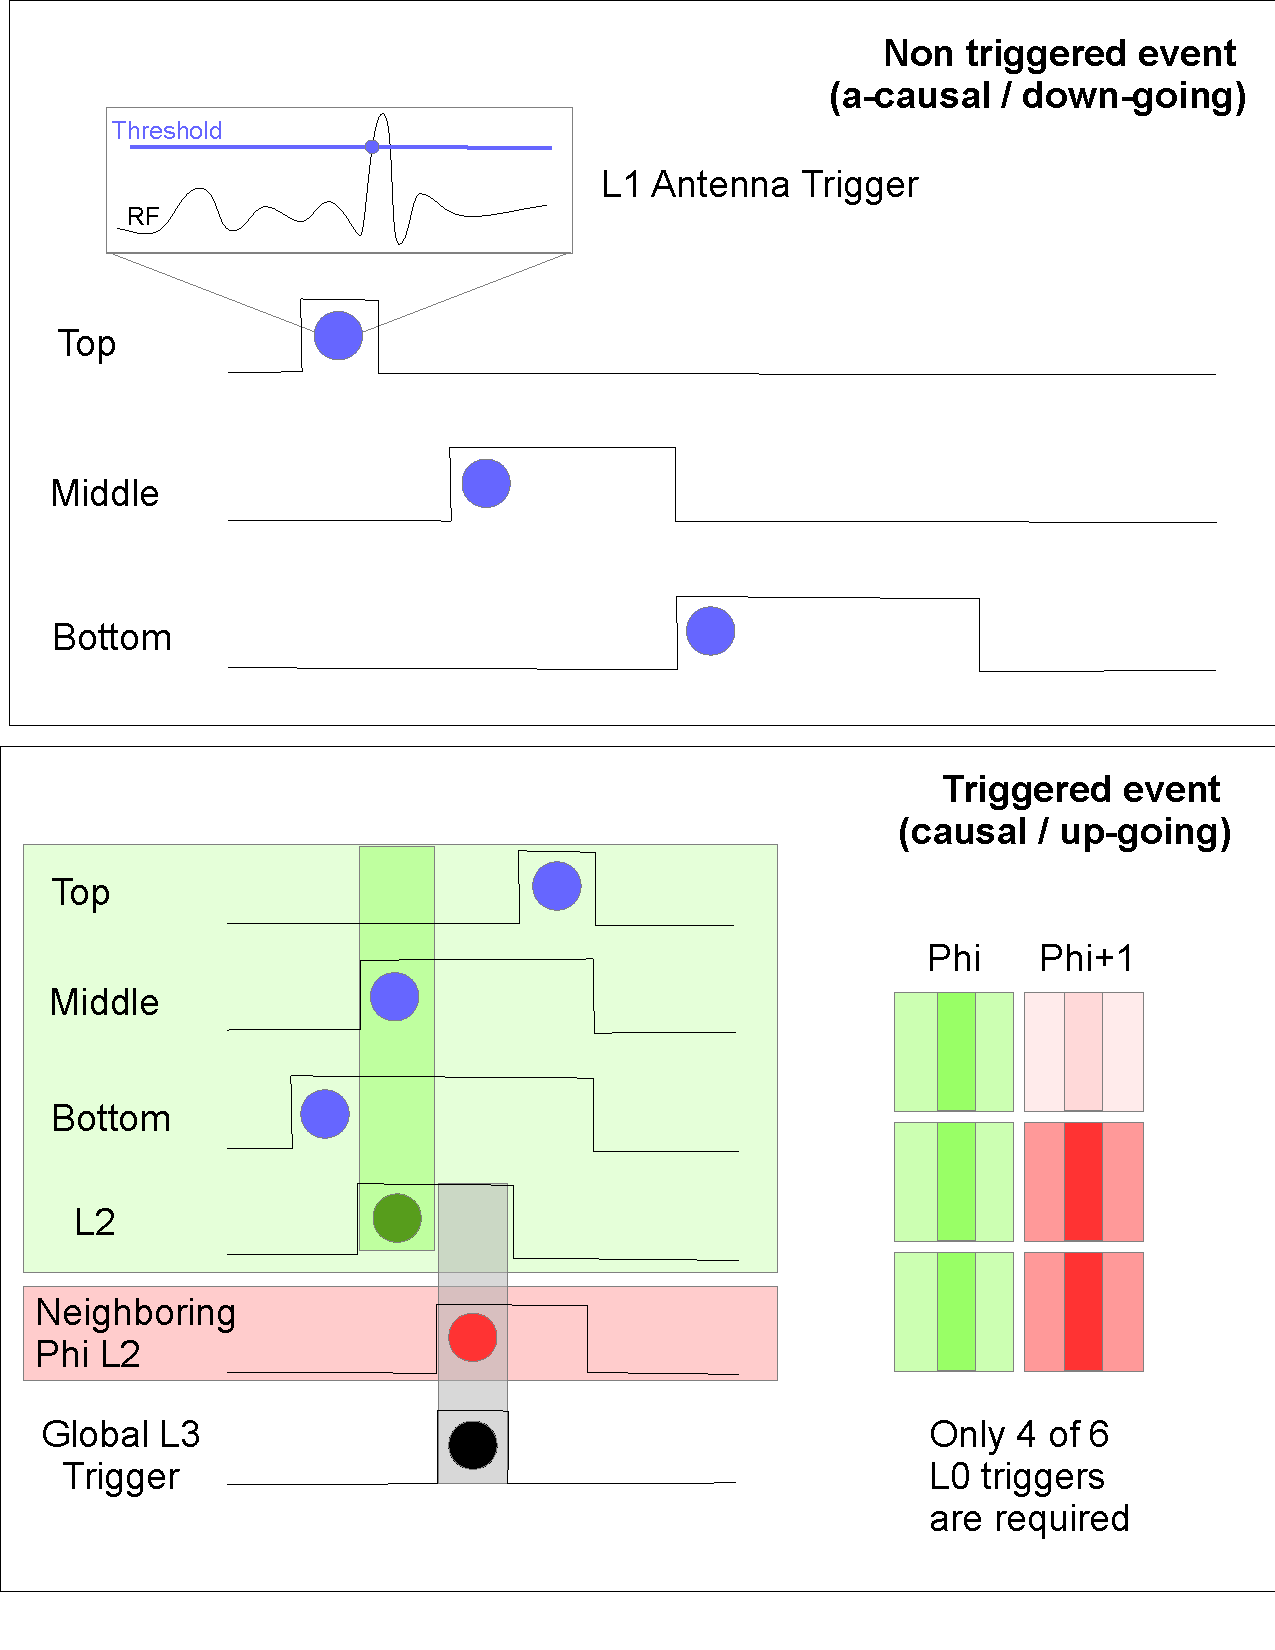
\includegraphics[height=0.8\textheight]{figures/triggerHeirarchy}
	\caption{A depiction of the trigger hierarchy for a non-triggered (top) and triggered (bottom) series of L0 triggers.  The blue dots denote an L0 trigger, and the green box represents the time of a L1  trigger.  Note the 4ns top ring window, the 12ns middle ring window, and the 16ns bottom ring window.  Two neighboring phi sectors with L1 triggers within a 8ns window cause a global trigger (black).  Note also that, though not the case of depicted event, only two of the three rings are required to be in coincidence leading to a 4 out of 6 channel L0 trigger in two neighboring phi sectors}
	\label{fig:trigPattern}
\end{figure}
		
	\subsection{L1 Trigger Window Delay Limitations}
		As the physical offsets between the rings of antennas exceeds one clock period for most of the angles of interest, it is possible to require a timing separation between the arrival of pulses between the separate antennas.  This modification, made between the ANITA2 and ANITA3 flights, decreases the incidental rate of the trigger, increasing the quality, while maintaining the signal rate and efficiency.  This is accomplished by generating a 16ns (four FPGA clock cycles) high logic pulse after a bottom ring antenna L0 trigger, a 12ns (three FPGA clock cycles) high logic pulse after a middle ring L0, and a 4ns window after a top ring L0.  The requirement for a L1 trigger is that two of these windowing pulses overlaps (see Figure \ref{fig:trigPattern}).  This has the unfortunate side effect of allowing the bottom ring of antennas to unfairly bais the system, as a noise L0 trigger generates a pulse with four times the time weight as one from the top ring, and is thus more likely to trigger the system.
		
	\subsection{L2 Multiple Phi Sector Trigger}
		The final L2 trigger is generated when two or more neighboring phi sectors report an L1 trigger within an 8 nanosecond window.  Once the L2 trigger is reported, the TURF board sends a HOLD command to all SURFS, which propagates to a single LAB and initializes a readout.

	\subsection{Phi Sector Masking}
		In the ANITA1 flight, it was discovered that noise sources on the continent and in the sky had the capability to dominate the trigger rate and effectively blind the entire payload despite a large fraction of the payload observing a thermal environment. To alleviate this issue, a system where an antenna or collection (phi sector) of antennas experiences a comparative increase in trigger rate in comparison to the rest of the payload, it will be excluded from forming the global system trigger.  This allows the instrument to continue observing quiet areas of the continent and increasing the total livetime of the system.  There are additional nuances to this subsystem, including the possibility of very high power noise (or signal) events continuing to leak into the back and side lobes of the antennas from non-masked phi sectors, that need to be taken into account when making a measurement of the total instrumented area for a flight.  During the ANITA3 flight, several unexpected in-band satellite CW signals caused the phi masking to be heavily utilized, which is discussed further in the Cosmic Ray Search chapter.
		
%	\subsection{Differences between previous ANITA flight trigger systems}
%		In addition to changing the number of antennas, each ANITA flight has made modifications to the trigger subsystem in an attempt to increase the efficiency and purity of measured events.
		
%		The ANITA1 instrument 
		
%		The ANITA2 instrument separated each signal channel into 3 frequency sub-bands and one full banded trigger within the SHORT boards, before the tunnel diodes.  The reasoning for this was that neutrino signals are full band; a signal with power dominating a single band would be enough to disqualify an event from being a true signal event.  The requirement for a global trigger was several (how many?) bands, in addition to the full band.  It was decided after the flight that this did not did not decrease the quantity of triggers by a significant amount, and the banding scheme was removed in favor of accommodating additional channels (ANITA2 did not trigger on Hpol and had 8 less antennas than ANITA3, so 56 additional trigger channels were required).  This had the unwanted effect of allowing CW signals from northern satellites to overwhelm the detector during the ANITA3 flight.
		
	\subsection{Unbiased triggers}
		Any waveform readout caused by a global trigger has the systematic bias that it passed the trigger selection parameters.  To measure the thermal noise environment during the flight, two triggers that were uncorrelated to the trigger circuit were employed.  These were a software trigger (also know as the soft-trig) that was issued by the CPU at a frequency of 1Hz, as well as a GPS synced 1Hz trigger controlled by the Pulse-Per-Second (PPS) output of the G12 GPS unit.
		
		All events captured by the payload were marked with a trigType integer that described the source of their trigger decision.  The GPS and soft-trig signals can be easily selected in this way by excluding RF triggers.
		
		
\section{RF Power Monitor}
	An additional digitization of the RF signal is done by a broad band radio frequency power detector circuit.  The fast waveform data only provides 200ns of non-triggered unbiased noise data per second (a 1Hz software trigger and a 1Hz gps trigger), so a monitor that digitized a larger fractional percentage of time was desired.  This was accomplished on the SURF board using a commercial RF power monitor IC that converted the RMS voltage of the input signal into a log-magnitude proportional DC output that was digitized by an ADC and read out with the slow read out housekeeping data.  This system, and the additional physics it provides is discussed at length in appendix A.

	
\section{GPS tracking and orientation sensors}
	Since the payload is attached to a free rotation balloon, the orientation and location of the payload was completely uncontrolled and thus needed to be constantly monitored.  This was primarily accomplished with two co-located ADU5 GPS heading receivers in conjunction with a single G12 GPS system.  These 9 total GPS antennas, read out once a second, provide a constant update for the location and orientation of the payload with a resolution of a fraction of a degree.
	
	\subsection{Magnetometer}
		In addition to the heading information provided by the GPS systems, a magnetometer was attached to the payload and used to measure the vector components of the magnetic field throughout the flight.  This system, coupled with a model for the geomagnetic field, could be used as a functional compass, assuming an accurate position, that would corroborate the pointing information returned by the GPS systems.
		
	\subsection{Sun Sensors}
		Many space borne experiments that require very high pointing and location precision, however are above the altitude where GPS has significant accuracy (is this a thing?), use star sensors to orient themselves.  ANITA's flight path over Antarctica during the austral summer, specifically the continual daylight, is able to use just one star to obtain accurate heading information.  With an accurate time and knowledge of the earth's rotation around the sun, one can use a simple pinhole camera and the four mounted angular sun sensors to determine the heading information for regions of time when the GPS is unavailable or unreliable.
		
\section{CPU, CPCI, and Data Readout}
	The custom LABRADOR digitizer ASICS and various control and command FPGAs are located on custom designed printed circuit boards (PCBs) connected to a central processing unit (CPU) over a compact peripheral component interconnect (cPCI) bus interface.  
	
\section{Data Storage and Telemetry}
	The most important piece of any experiment is the storage of the measurements for later analysis.  The quantity of data taken during flight saturates the hard-linked digital hardware used to read it out and store it, and thus it is not feasible to downlink the entirely of the stored information during flight.  This necessitates the recovery of the payload, or at least the storage vaults, immediately preceding the flight.

	\subsection{Redundant data storage}
		The storage requirements for the flight were met by three separate and unique digital storage formats.  This redundancy ensured that even in the event of a single failure the data from the flight would be preserved.  The first storage method was two identical Helium filled conventional spinning hard disk drives written to by the flight CPU over SATA.  The second method was a separately housed array of six solid state drives written to by a dedicated single board computer which received the flight data over an Ethernet link.  The third storage method, which ended being flown in an inactive state, was the RIFFRAFF handheld flash drive array; a complex system of microcontroller steered multiplexed commercial USB flash drives visible to the flight CPU.  During flight, a failure of the Ethernet link lead to the loss of the SSD array subsystem, leaving only the He Drive storage format intact.  Both drives survived the flight however, and two identical copies of data were recovered.
		In ANITA-III, the NTU device was a standalone CPU that connects with the flight CPU over ethernet and connected to six 1TB SSDs.  When one filled up, it would flip to the next.  It stopped communicating like a third of the way into the flight (probably because the ethernet power cable wiggled loose and all ethernet connectivity ceased), and was not ever required due to the success of the He drive system.
		
	
	\subsection{Telemetry}
		Downlink of data taken during flight and uplink of commands to change flight configuration are transmitted to and from ground receivers over several systems.  In order of decreasing data trasmission speed, they are the Line Of Sight (LOS) transmitter, an Iridium Pilot\textregistered Openport UDP link, a NASA Tracking and Data Relay Satellite System (TDRSS), and an Iridium\textregistered low rate downlink.  These systems allow in-flight diagnostics of the ANITA3 instrument, as well as an ability to make pre-defined alterations to instrument control configurations depending on need.  Shortly after flight, the Iridium Pilot\textregistered Openport link failed for unknown reasons.  However, the remaining systems were successful in allowing flight operators to debug and fix several issues that cropped up during the flight.
		
	\subsection{GPU prioritization}
		The data limitations of the various telemetry downlink systems allow only a fraction of the total data rate to be transmitted.  This limitation motivates a prioritization system in order to only send down events that pass a limited set of post-digitization analysis cuts.  This would allow a limited set of analyzable signals in the event of a catastrophic system failure or non-recovery of the payload.  The two major figures of merit for discriminating between incidental thermal noise events and impulsive signal-like events is the normalized peak height of an interferometric pointing map, and the peak of the Hilbert envelope of the coherently summed waveform for the respective map peak incidence angle.  These time-consuming, computationally intensive, physical baseline dependent, multiple channel correlation processes are nominally done offline in the analysis phase of the experiment, and is likewise further discussed in the analysis chapter of this thesis.  However, to accomplish the task in real time as events are streaming from the instrument, a Graphical Processing Unit (GPU) linked with the flight CPU was utilized to parallelize the computations and reduce any specific event readout's required processing time to that of the minimum instrument readout time.  These values were then used to determine a priority for each event and placed in an appropriate telemetry queue.  The main work on this system was done by Ben Strutt of University College London, and details on its operation and results can be found in his thesis at \cite{BenSThesis}.  Since the instrument was recovered, these computations are re-done for this thesis, and the priority value was not used.
		
	\subsection{Balloon}
		The ANITA instrument is suspended by a NASA zero pressure long duration high altitude balloon.  This balloon is cool.
			
			